\documentclass{clv2025}

\jvol{vv}
\jnum{nn}
\jyear{2026}
\jinfo{}
\renewcommand{\footmark}{}
\dochead{Position Paper}

\usepackage[T1]{fontenc}
\usepackage[american]{babel}
\usepackage{natbib}
\bibliographystyle{compling}
\usepackage{mathtools}
\usepackage{amssymb}
\usepackage{booktabs}
\usepackage{tabularx}
\usepackage{array}
\usepackage{graphicx}
\usepackage{xcolor}
\usepackage{tikz}
\usetikzlibrary{arrows.meta,positioning,calc}
\hypersetup{hidelinks}

\newcommand{\TC}{\textsc{TC}}
\newcommand{\LD}{\textsc{LD}}
\newcommand{\Hall}{\textsc{H}}
\newcommand{\SUP}{\textsc{SUP}}
\newcommand{\SV}{\textsc{SV}}
\newcolumntype{Y}{>{\raggedright\arraybackslash}X}
\newcolumntype{P}[1]{>{\raggedright\arraybackslash}p{#1}}

\definecolor{clrH}{RGB}{155,18,18}
\definecolor{clrLD}{RGB}{22,98,48}
\definecolor{clrB}{RGB}{22,52,125}
\definecolor{clrP}{RGB}{92,61,145}
\definecolor{clrO}{RGB}{170,91,24}
\definecolor{clrG}{RGB}{65,65,65}
\definecolor{bgB}{RGB}{245,247,254}
\tikzset{
  input/.style={rectangle,rounded corners=4pt,draw=gray!55,fill=gray!8,
    font=\small\itshape,text width=5.0cm,align=center,inner sep=6pt},
  decision/.style={rectangle,rounded corners=3pt,draw=clrB!55,fill=bgB,
    font=\small,text width=5.2cm,align=center,inner sep=6pt},
  verdict/.style={rectangle,rounded corners=3pt,draw=clrG,fill=gray!8,
    font=\small\bfseries\sffamily,inner xsep=7pt,inner ysep=4pt},
  verdictH/.style={verdict,draw=clrH,text=clrH,fill=clrH!7},
  verdictLD/.style={verdict,draw=clrLD,text=clrLD,fill=clrLD!7},
  arrow/.style={-{Stealth[length=5pt,width=3.5pt]},thick,color=gray!70!black},
  edge/.style={font=\scriptsize\sffamily,fill=white,inner sep=1.5pt},
  oracle/.style={rectangle,rounded corners=3pt,draw=clrO!60,fill=clrO!6,
    font=\scriptsize,text width=4.4cm,align=left,inner sep=5pt},
  slot/.style={rectangle,rounded corners=2pt,draw=clrB!40,fill=bgB,
    font=\scriptsize,align=center,inner sep=3pt},
  span/.style={rectangle,rounded corners=2pt,draw=gray!50,fill=gray!6,
    font=\scriptsize,text width=3.05cm,align=left,inner sep=4pt},
  claim/.style={rectangle,rounded corners=2pt,draw=gray!45,fill=white,
    font=\scriptsize,text width=3.05cm,align=left,inner sep=4pt},
  stage/.style={font=\scriptsize\sffamily\bfseries,color=clrG,anchor=east,align=right}
}

\title{Hallucination Is Contract-Relative: A Truth-Contract Framework for LLM Evaluation}
\runningtitle{Hallucination Is Contract-Relative}
\runningauthor{Carlesso et al.}

\author{Mathis Carlesso$^{1,2}$, Martino Lovisetto$^{2}$, El\H{o}d Egyed-Zsigmond$^{1}$, Pierre-Yves Genest$^{2}$, Stefan Duffner$^{1}$}

\affilblock{
  \affil{INSA Lyon, CNRS, LIRIS, UMR5205, Universit\'e Claude Bernard Lyon 1, 69621 Villeurbanne, France\\
  \quad \email{mathis.carlesso@insa-lyon.fr}}
  \affil{Alteca, 69100 Villeurbanne, France}
}

\begin{document}
\maketitle

\begin{abstract}
Hallucination in large language models is usually scored as a binary defect: a claim is either supported by evidence or it is not.
This framing works for narrow factual question answering, but it breaks down as soon as a task legitimately asks for something beyond the available evidence, such as a metaphor, a hypothesis, or a piece of fiction.
The same unsupported sentence can be a dangerous error in a medical answer, harmless in a poem, or exactly what a brainstorming or fiction-writing task requested.
We argue that hallucination should be judged against the task's \emph{truth contract} rather than against the sentence alone: what evidence the task is answerable to, what style it invites, and what kind of invention it permits.
This yields three claim-level labels instead of two: supported, hallucination, and licensed divergence, the last of which covers invention the task authorized.
Two claims with identical wording can deserve opposite verdicts once the task is taken into account, yet current evaluation practice rarely makes this task-dependence explicit.
We support this position with an author-coded mapping of forty widely used hallucination and creativity evaluation resources, which shows that factuality benchmarks and creative-writing benchmarks occupy separate corners of this space rather than testing the same underlying capability, and with a set of contrastive cases that make the resulting labeling consequences concrete.
On this basis, we lay out a research agenda for evaluation methods that make explicit what a task permits, so that reducing hallucination does not come at the cost of suppressing the invention that many tasks require.
\end{abstract}

\section{Introduction}\label{sec:intro}

Large language models (LLMs) can produce fluent claims that are unsupported by evidence or contradicted by known facts \citep{ji_survey_2023,huang_survey_2025}.
These errors limit the use of LLMs in high-stakes settings, therefore a large body of work aims to detect and reduce them \citep{lin_truthfulqa_2022,li_halueval_2023,wei_measuring_2024}.

However, generation beyond the available evidence is not always an error.
Fiction permits invention, whereas brainstorming and hypothesis generation may require claims that are not entailed by the available evidence \citep{franceschelli_creativity_2024,jiang_survey_2024,sui_confabulation_2024}.

A medical assistant should not invent a diagnosis.
A fiction-writing assistant must be able to invent characters and events.
The relevant question is therefore not only whether a statement is supported, but also whether the task permits departing from that support.

Many current evaluation protocols do not represent this distinction explicitly.
Factuality and faithfulness evaluations typically penalize unsupported claims under a fixed evidence source \citep{maynez_faithfulness_2020,bang_hallulens_2025}.
Creativity evaluations reward novelty and appropriateness, but they do not always test whether an apparently novel statement violates a factual constraint \citep{acar_creativity_2019,hou_creativityprism_2025}.
Consequently, two protocols can assign different claim labels to the same text because each  assumes a different task, emphasized by different prompts.

A second diagnostic problem concerns form rather than invention.
Stylistic foregrounding makes linguistic form salient through devices such as deviation, parallelism, metaphor, and unusual phrasing \citep{leech_short_style_1981,vanpeer_stylistics_2020}.
Some of these devices can change how a claim is expressed without adding a new factual commitment \citep{badathala_match_2023,jin_deep_2022}.
An evaluator that literalizes a metaphor, or reads surface unexpectedness as evidence of factual deviation, can therefore report a hallucination although the underlying claim remains supported.
The point is not that all current factuality systems make this error, but that many protocols do not expose the requested style level as a variable, so the error cannot be measured.

\paragraph{Our position}
Two terms carry the argument, and we fix them before using them further.
A \emph{claim} is a truth-conditional commitment attributed to the response: something the response puts forward as being the case, and which can therefore be checked against evidence.
A sentence may carry several claims, one, or none; ``the winter that would not lift'' asserts nothing checkable, while a single clause may commit to a date, a place, and a quantity at once.
A \emph{response span} $s$ is the stretch of text a claim is read off, and it is the unit an evaluator works with, because a response mixes spans that carry claims, spans that carry only style, and spans that carry neither.
Claims, not sentences and not responses, are what receives a label here.

Hallucination is not a context-free property of a sentence.
It is a claim-level label relative to the task's truth contract, which we write as $\TC(p)=(O_p,\sigma_p,\Gamma_p,\mu_p)$ and define in full in \S\ref{sec:framework}.
Its fields are the reference evidence $O_p$, the requested style level $\sigma_p$, and two permission fields: the scope $\Gamma_p$ within which unsupported content is allowed, and the \emph{epistemic presentation} $\mu_p$ it must carry.
By epistemic presentation we mean the marking that signals the status of what is asserted, such as a hedge, a hypothesis marker, or a declared fictional frame.
We follow the standard convention in which a model maps a prompt $x$ to a response $y$, and we keep both symbols with their usual meaning.
The contract, however, is not indexed on $x$.
It is indexed on the \emph{task context} $p$, which contains $x$ together with the applicable system instructions, such as a fixed register, the domain constraints, such as a specified knowledge base, and any attached evidence.
Two identical prompts issued under different system instructions carry different contracts, which is why $p$ rather than $x$ is the right index, and why we introduce a separate symbol instead of overloading $x$.
An entailed claim is labeled \SUP\ (supported).
An unsupported claim is labeled \Hall\ if it falls outside $\Gamma_p$ or fails $\mu_p$; an evidence-unknown claim is labeled \LD\ if the scope permits it and its presentation satisfies the contract.
These labels apply to individual claims; assessing a complete response requires a separate aggregation step that this paper does not fix.
The contract does not change what is true.
It determines whether the model's departure from the relevant evidence violates the task.

Figure~\ref{fig:flip} illustrates this position.
The figure uses a constructed example: \emph{Verdier} is an invented name introduced here, not a quotation from a dataset.
It follows one claim wording extracted from a hypothetical model response and shows that its label depends on the prompt and truth contract.
The wording is fixed, but each prompt establishes a different discourse frame, so the two occurrences do not express the same contextualized claim.

\begin{figure}[t]
\centering
\resizebox{0.94\linewidth}{!}{%
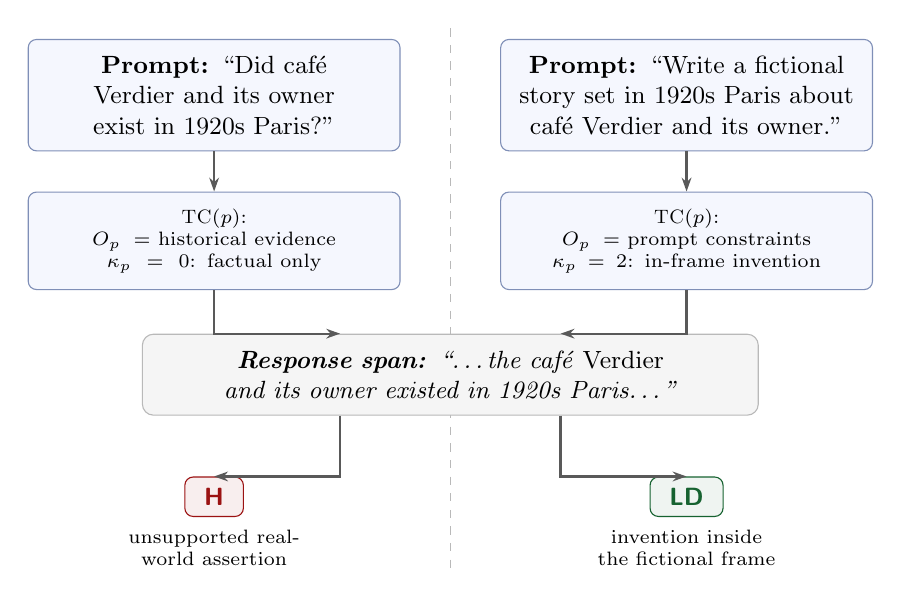
\begin{tikzpicture}[x=1cm,y=1cm]
  \draw[dashed,gray!55] (0,0.85) -- (0,-6.05);
  \node[decision,text width=4.3cm] (qa) at (-3.0,0)
    {\textbf{Prompt:} ``Did caf\'e Verdier and its owner exist in 1920s Paris?''};
  \node[decision,text width=4.3cm] (fi) at (3.0,0)
    {\textbf{Prompt:} ``Write a fictional story set in 1920s Paris about caf\'e Verdier and its owner.''};
  \node[decision,text width=4.3cm,font=\scriptsize] (tcqa) at (-3.0,-1.85)
    {$\TC(p)$:\\$O_p=$ historical evidence\\$\kappa_p=0$: factual only};
  \node[decision,text width=4.3cm,font=\scriptsize] (tcfi) at (3.0,-1.85)
    {$\TC(p)$:\\$O_p=$ prompt constraints\\$\kappa_p=2$: in-frame invention};
  \node[input,text width=7.4cm] (s) at (0,-3.55)
    {\textbf{Response span:} ``\dots the caf\'e \emph{Verdier} and its owner existed in 1920s Paris\dots''};
  \node[verdictH] (h) at (-3.0,-5.10) {\Hall};
  \node[verdictLD] (ld) at (3.0,-5.10) {\LD};
  \node[font=\scriptsize,align=center,text width=3.7cm] at (-3.0,-5.75)
    {unsupported real-world assertion};
  \node[font=\scriptsize,align=center,text width=3.7cm] at (3.0,-5.75)
    {invention inside the fictional frame};
  \draw[arrow] (qa) -- (tcqa);
  \draw[arrow] (fi) -- (tcfi);
  \draw[arrow] (tcqa.south) |- ($(s.north)+(-1.4,0)$);
  \draw[arrow] (tcfi.south) |- ($(s.north)+(1.4,0)$);
  \draw[arrow] ($(s.south)+(-1.4,0)$) |- (h.north);
  \draw[arrow] ($(s.south)+(1.4,0)$) |- (ld.north);
\end{tikzpicture}}
\caption{\textbf{One response wording, two contract-dependent labels.}
The same constructed response wording is evaluated under two prompts, each read against its own truth contract $\TC(p)$.
Under the historical-QA prompt it is an unsupported real-world assertion and receives \Hall\ as label; under the fiction-writing prompt it is an in-frame invention permitted by $\Gamma_p$ and receives \LD\ as label.
Strictly, each prompt changes the contextualized claim, so the figure shows contract dependence, not a contradiction about one fixed proposition.
Both labels are claim-level, not verdicts for the complete response.}
\label{fig:flip}
\end{figure}

\paragraph{Evidence and scope}
We support the position in two ways.
First, we map forty hallucination and creativity evaluation resources against the components of the proposed contract (full list in Appendix~\ref{app:mapping}).
This mapping is purposive and author-coded: it identifies a pattern within our sample, not a prevalence estimate for the broader literature.
Second, we apply the labeling rule to five worked cases that vary, in turn, the reference evidence, the discourse frame, the required epistemic presentation, the permission scope, and finally the requested style level, holding the claims fixed, to test whether a marked realization changes which claims an evaluator reads off a span.
These cases illustrate the intended behavior of the labeling rule defined in \S\ref{sec:framework} but do not establish annotation reliability or completeness.

\paragraph{Contributions}
This position paper makes three contributions.
First, it introduces the truth contract $\TC(p)=(O_p,\sigma_p,\Gamma_p,\mu_p)$.
The contract separates reference evidence, requested style level, permission scope, and required epistemic presentation, and distinguishes \Hall\ from \LD.
Second, it maps a sample of factuality and creativity protocols to identify where task permissions and form-conditioned factuality checks remain implicit.
Third, it proposes a research agenda for contract-aware benchmarks and mitigation methods that reduce \Hall\ without suppressing \LD\ or factual stylistic creativity.

\paragraph{Plan of the paper}
Section~\ref{sec:framework} defines the truth contract and the claim-level labeling rule.
Section~\ref{sec:related} situates the framework against hallucination taxonomies, faithfulness and alignment work, and claim-extraction methods; existing taxonomies classify \emph{where} a mismatch originates, whereas the contract asks \emph{whether the task authorized} the departure, which is a different question and the reason we introduce a third label.
Section~\ref{sec:audit} reports the resource mapping, Section~\ref{sec:cases} applies the rule to five worked cases, and Sections~\ref{sec:agenda}--\ref{sec:discussion} set out the research agenda and its limits.

\section{Truth Contracts and Claim-Level Labels}\label{sec:framework}

\subsection{Overview: from a response span to a label}

Figure~\ref{fig:prompt-to-claim} carries one constructed example through the whole procedure, and we reuse it as a running example for the rest of the paper.
A museum-panel prompt attaches an archive extract as the reference evidence, asks for a vivid register, and states that where the extract is silent the response may add a plausible reconstruction provided it is marked as conjecture.
Those three requests are exactly the three components of the contract: the extract fixes what counts as support, the register fixes the requested style level, and the conjecture clause fixes what may be invented, where, and how it must be signaled.

The response is then read span by span.
A span reporting the admission figure recorded in the extract yields one canonical claim that the extract entails, so it receives \SUP.
A span rendering the mask order as a metaphor expresses the same commitment in marked form: the claim is still entailed, and the span additionally carries an \SV\ (\emph{stylistic variation}) flag, because the requested style neither creates nor excuses a truth-conditional claim.
A hedged span about school closures is not settled by the extract, but it stays within the permitted subject matter and is marked as conjecture, so it receives \LD.
A span asserting that a named hospital director concealed the death toll is also unsettled by the extract, yet it concerns an identified individual outside the permitted subject matter \emph{and} is asserted without the required marking, so it receives \Hall.
One prompt, one contract, one response, four different labels.

The example follows one fixed chain, used throughout the paper:
\emph{response $\rightarrow$ response span $\rightarrow$ contextualized claim $\rightarrow$ canonical claim $\rightarrow$ evidence state $\rightarrow$ contract-relative label}.
Table~\ref{tab:symbols} lists the objects used in the formal definition, and each of them appears in Figure~\ref{fig:prompt-to-claim} at the stage where it acts.

\begin{figure}[!t]
\centering
\resizebox{0.96\linewidth}{!}{%
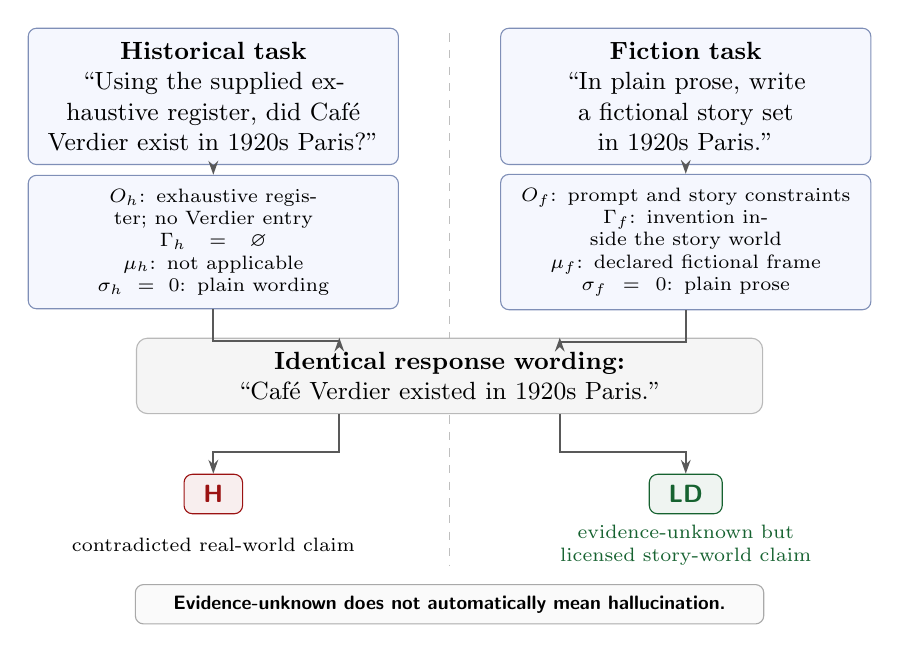
\begin{tikzpicture}[x=1cm,y=1cm]
  \tikzset{
    taskbox/.style={
      decision,text width=4.35cm,minimum height=1.25cm,
      font=\small,inner sep=5pt},
    contractbox/.style={
      decision,text width=4.35cm,minimum height=1.55cm,
      font=\scriptsize,inner sep=5pt},
    sharedspan/.style={
      input,text width=7.6cm,minimum height=0.95cm,
      font=\small,inner sep=5pt},
    outcome/.style={
      font=\scriptsize,align=center,text width=3.75cm}
  }

  \draw[dashed,gray!50] (0,0.8) -- (0,-5.95);

  \node[taskbox] (historical) at (-3.0,0)
    {\textbf{Historical task}\\
     ``Using the supplied exhaustive register, did Caf\'e Verdier exist in 1920s Paris?''};
  \node[taskbox] (fiction) at (3.0,0)
    {\textbf{Fiction task}\\
     ``In plain prose, write a fictional story set in 1920s Paris.''};

  \node[contractbox] (tch) at (-3.0,-1.85)
    {$O_h$: exhaustive register; no Verdier entry\\
     $\Gamma_h=\varnothing$\\
     $\mu_h$: not applicable\\
     $\sigma_h=0$: plain wording};
  \node[contractbox] (tcf) at (3.0,-1.85)
    {$O_f$: prompt and story constraints\\
     $\Gamma_f$: invention inside the story world\\
     $\mu_f$: declared fictional frame\\
     $\sigma_f=0$: plain prose};

  \node[sharedspan] (span) at (0,-3.55)
    {\textbf{\upshape Identical response wording:}\\
     ``Caf\'e Verdier existed in 1920s Paris.''};

  \node[verdictH] (hall) at (-3.0,-5.05) {\Hall};
  \node[verdictLD] (licensed) at (3.0,-5.05) {\LD};
  \node[outcome] at (-3.0,-5.70)
    {contradicted real-world claim};
  \node[outcome,text=clrLD] at (3.0,-5.70)
    {evidence-unknown but licensed story-world claim};

  \coordinate (spanlefttop) at ($(span.north)+(-1.4,0)$);
  \coordinate (spanrighttop) at ($(span.north)+(1.4,0)$);
  \coordinate (spanleftbot) at ($(span.south)+(-1.4,0)$);
  \coordinate (spanrightbot) at ($(span.south)+(1.4,0)$);

  \draw[arrow] (historical.south) -- (tch.north);
  \draw[arrow] (fiction.south) -- (tcf.north);
  \draw[arrow]
    (tch.south) -- ++(0,-0.40)
    -| (spanlefttop);
  \draw[arrow]
    (tcf.south) -- ++(0,-0.40)
    -| (spanrighttop);
  \draw[arrow]
    (spanleftbot) -- ++(0,-0.48)
    -| (hall.north);
  \draw[arrow]
    (spanrightbot) -- ++(0,-0.48)
    -| (licensed.north);

  \node[
    rectangle,rounded corners=3pt,draw=clrG!45,fill=gray!4,
    font=\scriptsize\sffamily\bfseries,align=center,
    text width=7.7cm,inner sep=4pt
  ] at (0,-6.45)
    {Evidence-unknown does not automatically mean hallucination.};
\end{tikzpicture}%
}
\caption{\textbf{Identical wording under two truth contracts.}
The response span yields a real-world claim in the historical task and a story-world claim in the fiction task.
The historical claim receives \Hall\ because the task treats the register as complete and the missing entry contradicts the claim.
The fictional claim receives \LD\ because its detail is evidence-unknown, but story-world invention lies inside $\Gamma_f$ and the declared fictional frame satisfies $\mu_f$.
Both tasks request plain wording, so style does not explain the label difference.
\LD\ denotes contractual permission, not a benign hallucination or a judgment of truth, quality, or safety.}
\label{fig:prompt-to-claim}
\end{figure}


\begin{table}[t]
\centering
\footnotesize
\setlength{\tabcolsep}{4pt}
\renewcommand{\arraystretch}{1.08}
\caption{\textbf{Core objects in the truth-contract framework.}}
\label{tab:symbols}
\begin{tabularx}{\linewidth}{@{}P{0.24\linewidth}Y@{}}
\toprule
\textbf{Symbol} & \textbf{Meaning}\\
\midrule
$x,y$ & prompt and complete response, in the usual sense\\
$p,s$ & task context ($x$ plus system instructions, domain constraints, attached evidence) and response span\\
$O_p,\sigma_p$ & reference evidence and requested style level\\
$\Gamma_p,\mu_p$ & permission scope and required epistemic presentation\\
$\kappa_p$ & ordinal summary of $(\Gamma_p,\mu_p)$; not consulted by the labeling rule\\
$\mathcal C(s,p),c^*$ & contextualized claims recovered from $s$, and one canonical claim\\
$\widehat\sigma(s,p),z(s,p)$ & observed style level and binary \SV\ flag\\
$E(c^*,O_p)$ & evidence state relative to $O_p$\\
$V(c^*\mid p),R(y\mid p)$ & claim label and separate response-level assessment\\
\bottomrule
\end{tabularx}
\end{table}
\subsection{The truth contract}

\paragraph{Truth contract (\TC)}
For a task context $p$, the truth contract is
\[
  \TC(p)=(O_p,\sigma_p,\Gamma_p,\mu_p).
\]
The fields answer different questions: what supports a claim ($O_p$), what style the task requests ($\sigma_p$), and, when the reference evidence settles nothing, what content the task nonetheless permits ($\Gamma_p$) and how that content must be signaled ($\mu_p$).
We refer to $\Gamma_p$ and $\mu_p$ together as the \emph{permission fields}, since they answer the same underlying question and are the two fields the labeling rule consults.
As stated in \S\ref{sec:intro}, $p$ denotes the task context and not the prompt $x$ alone.
We drop the subscript $p$ when the task is clear from context.

\paragraph{Reference evidence ($O_p$)}
$O_p$ is the reference information against which a claim is evaluated, such as a source document, retrieval set, database, gold labels, a specified external source, or declared fictional-frame constraints.
The phrase ``world knowledge'' is only a shorthand; reproducible evaluation requires a concrete evidence source or an explicit adjudication procedure \citep{ji_survey_2023,bang_hallulens_2025}.

\paragraph{Permission fields ($\Gamma_p$ and $\mu_p$)}
Two fields specify what a response may do when $O_p$ does not entail a claim:
\begin{itemize}
  \item $\Gamma_p$: the \emph{permission scope}, meaning the topics, entities, or fictional world in which evidence-unknown content may be introduced;
  \item $\mu_p$: the \emph{required epistemic presentation}, meaning how the response must signal the status of that content, for example with a hedge, an explicit hypothesis marker, or a declared fictional frame. We write $\mu$ for the \emph{marking} the field requires, and use ``marking'' as the short name for it throughout.
\end{itemize}
The two answer different questions and should not be read as duplicates.
$\Gamma_p$ bounds what evidence-unknown content a task may introduce; $\mu_p$ governs how that content must be signaled once introduced.
A factual-only task has an empty permission scope: every truth-conditional claim must be supported wrt. $O_p$.
For $\Gamma_p$, consider a medical brainstorming task that permits possible diagnoses but not invented drug doses; the diagnosis space is inside the scope, whereas invented treatment content, such as drug doses, is outside of it.
For $\mu_p$, ``this may be early Lyme disease, but testing is required'' satisfies a request to mark uncertainty, while ``this is early Lyme disease'' does not.
In fiction, the declared story frame can satisfy $\mu_p$ for invented characters and events, but $\Gamma_p$ may still exclude fabricated real-world claims about named people \citep{searle_logical_1975}.

\paragraph{Permission level ($\kappa_p$), a derived summary}
Describing a task by two fields is precise but inconvenient when the point is to compare whole benchmarks, and a protocol often fixes both fields implicitly without stating either.
We therefore write $\kappa_p\in\{0,1,2\}$ for a coarse ordinal summary of the pair $(\Gamma_p,\mu_p)$:
\begin{itemize}
  \item $\kappa_p=0$: the scope is empty, so no marking requirement arises and the task is factual only;
  \item $\kappa_p=1$: the scope is narrow and bounded by subject matter, and content introduced within it must carry an explicit marking;
  \item $\kappa_p=2$: the scope is coextensive with a declared frame, and the declaration of that frame is itself what satisfies the marking requirement.
\end{itemize}
$\kappa_p$ summarizes both fields because the two co-vary in practice: a task that widens what may be invented also changes what counts as adequately signaling it, and a declared fictional frame licenses content and marks it in one move.
This is why $\kappa_p=1$ is glossed as ``limited \emph{and explicitly marked} divergence'' without that gloss duplicating $\mu_p$: the level records that a marking requirement exists, whereas $\mu_p$ states which marking discharges it.

$\kappa_p$ is \emph{not} a field of the contract, and the labeling rule of \S\ref{sec:framework} never consults it.
It is a compression of two fields into one number, so it loses exactly what the rule needs: which topics are in scope, and which marking counts.
We retain it for one purpose, namely that a three-level value can be assigned to a resource that never states its scope or its marking requirement separately, which is what makes the cross-resource comparison of \S\ref{sec:audit} possible at all.
The scale orders only the breadth of permitted departure, not quality, creativity, or factuality; in particular, limited speculation and declared fiction carry different commitments even where both are marked.

\subsection{Requested style levels}

The truth contract distinguishes three requested style levels, $\sigma_p\in\{0,1,2\}$:
\begin{itemize}
  \item $\sigma_p=0$ (neutral/literal): minimal rhetorical transformation and no salient authorial voice;
  \item $\sigma_p=1$ (moderately marked): local metaphor, register shift, or a light stylistic voice while the intended claims remain transparent;
  \item $\sigma_p=2$ (strongly marked): sustained figurative language, a salient voice, or substantial stylistic transformation.
\end{itemize}
The levels rank the degree of stylistic marking.
They do not rank creativity or factuality, and they do not grant permission to invent.
The levels approximate \emph{stylistic marking}, defined here as a noticeable departure from neutral wording through deviation or repetition \citep{leech_short_style_1981,vanpeer_stylistics_2020}.
This operational notion is related to foregrounding in stylistics.
Metaphor is a central semantic case, but marking may also be lexical, syntactic, phonological, or discourse-level.
Surface unexpectedness is therefore not, by itself, evidence of factual error.
Style is multi-dimensional, so this three-level scheme is a working discretization rather than a validated universal scale \citep{kang_style_2021,jin_deep_2022}.
The boundaries, especially between $\sigma_p=1$ and $\sigma_p=2$, require empirical validation.
Shared-task settings that already control register while holding content fixed, such as text simplification with a specified target audience \citep{simpletext_task2_2026}, offer the closest existing calibration point for such a validation.

The requested style level $\sigma_p$ must be distinguished from the observed style level $\widehat\sigma(s,p)$ in an output span $s$.
For example, a prompt can request $\sigma_p=2$ while the model produces neutral prose with $\widehat\sigma(s,p)=0$.
This mismatch is a style-compliance error, not a hallucination.

\paragraph{Where each component acts}
The three components of the contract are not redundant, and the reason is that they act at two different stages of the same pipeline.
Claim recovery comes first: interpreting a span $s$ in task context $p$ to obtain the contextualized claims $\mathcal C(s,p)$ and their canonical restatements.
Labeling comes second: comparing each canonical claim with $O_p$ and checking it against the permission fields.
\emph{$\sigma_p$ acts at the recovery stage; $O_p$, $\Gamma_p$, and $\mu_p$ act at the labeling stage.}
This is why $\sigma_p$ does not appear in the labeling rule of \S\ref{sec:framework} while still belonging to the contract: a requested style level changes which claims an evaluator recovers from a span, and therefore which objects the labeling rule ever sees, without changing how any recovered claim is scored.
Reading the absence of $\sigma_p$ from the labeling rule as evidence that style is extraneous mistakes a two-stage pipeline for a one-stage one.
The requested style level guides the interpretation of a span, while the observed style level records the form that the model produced.

Style belongs in the contract for the same reason evidence and permission do: tasks routinely specify a register, such as a memo, a poem, or a terse answer, and the contract should make that request explicit rather than leave it implicit in the prompt.
$\sigma_p$ does not authorize unsupported content on its own; that is $\kappa_p$'s role.
Tracking $\sigma_p$ separately from $\kappa_p$ guards against two failure modes: an evaluator that flags a stylistic departure as \Hall\ although no factual commitment was violated, and a stylistic departure that masks a real $\kappa_p$ violation underneath an acceptable surface form.

This concern is not hypothetical.
Claim extractors, entailment systems, and semantic metrics may react differently to literal and figurative realizations of the same claim \citep{chen_menli_2023,aynetdinov_semscore_2024,lai_multidimensional_2023,pauli_mind_2025}, and LLM-judge alignment benchmarks show the same asymmetry at a larger scale: judges penalize a sarcastic tone far more heavily than a factual error, and terse responses can even be scored below verbose incorrect ones \citep{feuer_style_2025}.
As a result, stylistic form can change which claims an evaluator extracts, verifies, and rewards, even though $\sigma_p$ does not authorize new content by itself.

\subsection{Unit of analysis and span typing}

We use a claim-level unit because a response may mix supported, unsupported, and non-claim material \citep{min_factscore_2023,bayat_factbench_2024}.
Let $s$ denote a response span.
Interpreting $s$ in task context $p$ yields a set of contextualized truth-conditional claims $\mathcal C(s,p)$.
The same wording can therefore yield different claims depending on discourse frame, as in the historical-QA and fiction-writing pair worked through in Figure~\ref{fig:flip}.
For verification, an annotator restates each recovered claim as a neutral \emph{canonical claim} $c^*$ while preserving its factual commitment.

The evaluator also records the observed style level $\widehat\sigma(s,p)\in\{0,1,2\}$ and a binary \SV\ flag $z(s,p)\in\{0,1\}$ for an independently identifiable stylistic contribution.
Together, $\mathcal C(s,p)$ and $z(s,p)$ define four span types:
\begin{itemize}
  \item \emph{other}: $\mathcal C=\varnothing$ and $z=0$; the span is outside claim and style evaluation;
  \item \emph{SV-only}: $\mathcal C=\varnothing$ and $z=1$; the span keeps \SV, but no claim is verified;
  \item \emph{claim-only}: $\mathcal C\neq\varnothing$ and $z=0$; each recovered claim is verified;
  \item \emph{mixed}: $\mathcal C\neq\varnothing$ and $z=1$; the span keeps \SV\ while each recovered claim is verified.
\end{itemize}
Metaphor is not automatically removed from factual evaluation.
We annotate a metaphorical span as mixed when annotators recover both truth-conditional content and an independently identifiable stylistic contribution.
Some metaphors also introduce implicatures or new claims; those claims must be extracted and verified.

Canonical matching supports controlled comparisons across styles.
When two neutral paraphrases express the same factual commitment, annotators match them one-to-one before comparing evidence states and labels.
Appendix~\ref{app:diagnostics} gives the formal stability test.
The observed style levels and \SV\ flags may differ across matched variants.
An evaluator can fail at three stages.
It may drop a recoverable claim, convert stylistic material into a spurious claim, or change the label of an already matched canonical claim.
This requirement applies only to claim-preserving variants.
For models, the target capability is to produce stylistically creative yet factually grounded output whenever the permission fields require grounding.
Failure to produce the requested style level is an instruction-following error, whereas adding an unsupported claim under a factual-only contract is a truth-contract violation.

\subsection{Evidence state and claim label}

For every canonical claim $c^*$, record the evidence relation
\[
E(c^*,O_p)\in\{\textsc{entailed},\textsc{contradicted},\textsc{unknown}\}.
\]
The last value means that $O_p$ neither supports nor contradicts the claim; it is not a statement about all possible knowledge.
Evidence state alone does not determine the contractual claim label.

The \textsc{unknown} state carries a measurement risk that we state explicitly.
It aggregates genuine indeterminacy, retrieval failure, and claims outside the domain that $O_p$ covers, and under a permissive contract all three route to \LD.
A verification pipeline that under-retrieves therefore produces more \LD\ and appears more permissive-friendly than it is, which is an incentive problem rather than an annotation error.
Reporting \LD\ without reporting retrieval coverage over $O_p$ is not sufficient; separating the three sources is part of the pipeline-diagnosis agenda of \S\ref{sec:agenda}.

Let $L(c^*,\Gamma_p)\in\{0,1\}$ indicate whether $c^*$ is permitted within the scope $\Gamma_p$.
Let $D(c^*,s,\mu_p)\in\{0,1\}$ indicate whether span $s$ presents $c^*$ as required by $\mu_p$.
Each function receives exactly the field it tests, which is why $\kappa_p$ appears in neither.
Then
\[
V(c^*\mid p)=
\begin{cases}
\SUP & \text{if }E(c^*,O_p)=\textsc{entailed},\\[1mm]
\LD & \text{if }E(c^*,O_p)=\textsc{unknown},\ L=1,\ D=1,\\[1mm]
\Hall & \text{otherwise.}
\end{cases}
\]
\SUP\ means \emph{supported}: $O_p$ entails the claim.
\Hall\ means \emph{hallucination}: the claim is contradicted, or it is evidence-unknown without the required permission, scope, or presentation.
\LD\ means \emph{licensed divergence}: $O_p$ does not establish the claim, but the claim lies inside $\Gamma_p$ and is presented as $\mu_p$ requires.
An \LD\ label records contractual permission, not proof that the claim is true relative to $O_p$.

By default, a claim that contradicts $O_p$ receives \Hall.
For fiction, $O_p$ includes the declared fictional frame and its constraints; disagreement with the real world alone does not make an in-frame invention contradicted.
If an entailed claim violates a requested hedge or style, it remains \SUP\ but is additionally flagged with a task-compliance error.
\paragraph{Usefulness is a separate score}
Usefulness $U(c^*,p)$ is a task-dependent score reported over \LD\ claims only.
It answers a question the labeling rule deliberately does not ask: given that the contract authorized this divergence, was the divergence any good?
We do not propose a new measurement instrument for it.
The relevant instruments already exist and are task-specific: appropriateness judgments in creativity assessment, where novelty is scored jointly with fit to the task rather than alone \citep{acar_creativity_2019,franceschelli_creativity_2024}, and reader-facing quality judgments for generated narrative and explanatory text \citep{marco_reader_2025,chakrabarty_art_2024}.
What the contract adds is the ordering: permission is evaluated first and usefulness second, over the claims that permission has already admitted.
$U$ is therefore narrower than general response-to-prompt alignment, which this paper does not score, and narrower than response quality, which mixes usefulness with coverage and style compliance.
A low usefulness score does not change \LD\ into \Hall; an uninteresting authorized invention is a weak answer, not a hallucination.

An explicit refusal or a statement such as ``the available evidence is insufficient'' is evaluated as a meta-claim about the evidence.
It is not automatically treated as asserting the embedded unsupported claim.
This distinction prevents calibrated abstention from being mislabeled as hallucination.

\paragraph{Claim labels versus response-level assessment}
The rule above returns one claim-level label $V(c_i^*\mid p)$ for each canonical claim $c_i^*$ recovered from a response $y$.
It does not by itself return a verdict for the complete response.
Current evaluation methods often aggregate claim-level results with a proportion, mean score, or binary rule such as whether any error occurs \citep{min_factscore_2023,bayat_factbench_2024}.
These aggregations answer different questions: one severe \Hall\ may matter more than several minor supported claims, while a creative response can contain no \Hall\ yet still provide too little useful \LD.
We write $R(y\mid p)$ for a contract-aware response-level assessment that combines these claim-level outcomes.
Its aggregation rule should state how it combines claim labels with coverage, severity, usefulness, and style compliance under $\TC(p)$; designing that rule is an open research problem.
Figure~\ref{fig:decision} summarizes the full procedure, from response span to claim-level label to this open response-level step.


\begin{figure*}[t]
\centering
\resizebox{0.95\linewidth}{!}{%
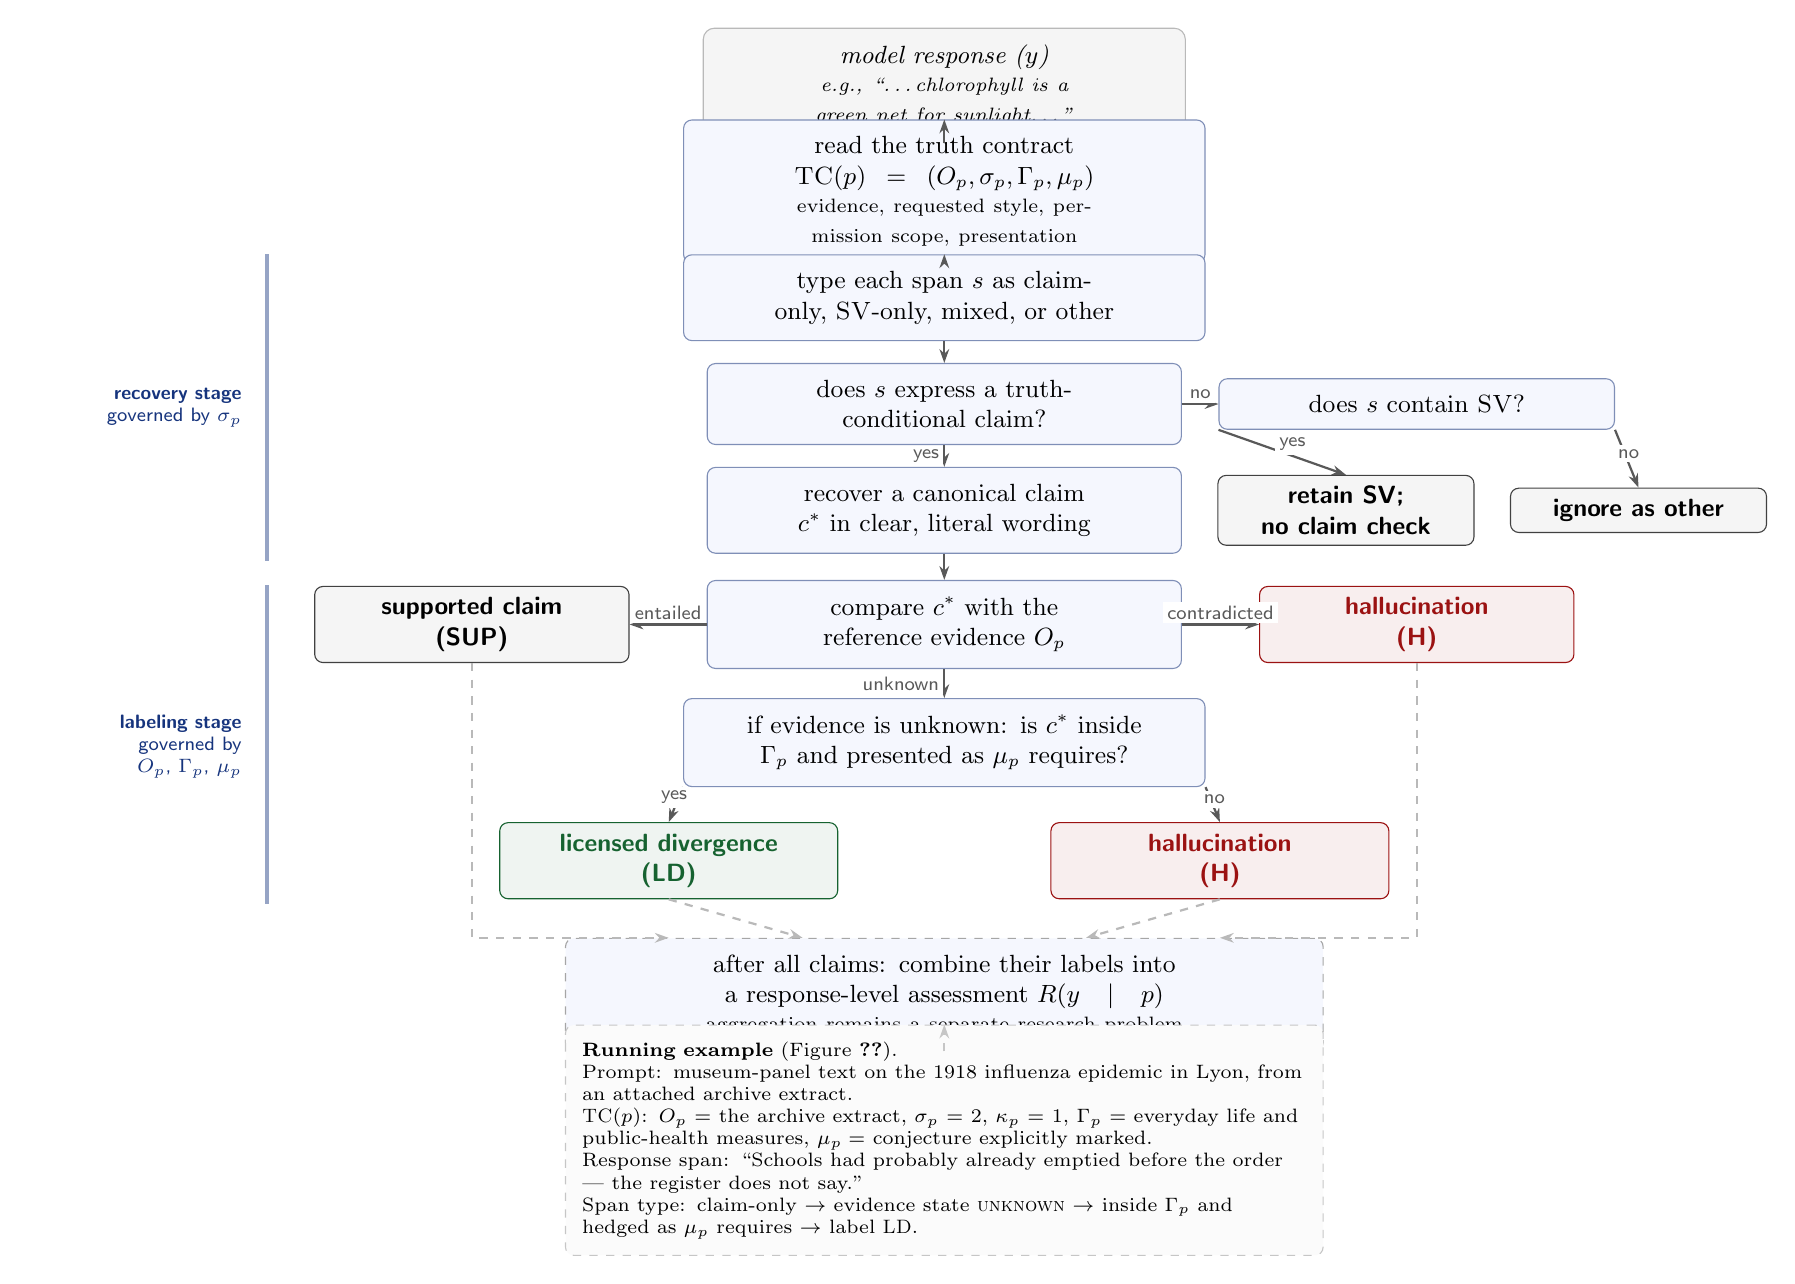
\begin{tikzpicture}[x=1cm,y=1cm]
  \node[input,text width=5.7cm] (response) at (0,0)
    {model response ($y$)\\[-1pt]
     {\scriptsize e.g., ``\dots chlorophyll is a green net for sunlight\dots''}};

  \node[decision,text width=6.2cm] (contract) at (0,-1.35)
    {read the truth contract $\TC(p)=(O_p,\sigma_p,\Gamma_p,\mu_p)$\\[-1pt]
     {\scriptsize evidence, requested style, permission scope, presentation}};

  \node[decision,text width=6.2cm] (label) at (0,-2.70)
    {type each span $s$ as claim-only, \SV-only, mixed, or other};

  \node[decision,text width=5.6cm] (hasclaim) at (0,-4.05)
    {does $s$ express a truth-conditional claim?};

  \node[decision,text width=4.6cm] (hassv) at (6.0,-4.05)
    {does $s$ contain \SV?};

  \node[decision,text width=5.6cm] (plainclaim) at (0,-5.40)
    {recover a canonical claim $c^*$ in clear, literal wording};

  \node[
    verdict,
    text width=2.9cm,
    inner xsep=5pt,
    align=center,
    right=0.45cm of plainclaim
  ] (styleonly)
    {retain \SV;\\no claim check};

  \node[
    verdict,
    text width=2.9cm,
    inner xsep=5pt,
    align=center,
    right=0.45cm of styleonly
  ] (other)
    {ignore as other};

  \node[decision,text width=5.6cm] (evidence) at (0,-6.85)
    {compare $c^*$ with the reference evidence $O_p$};

  \node[verdict,text width=3.5cm,align=center] (sup) at (-6.0,-6.85)
    {supported claim\\(\SUP)};

  \node[verdictH,text width=3.5cm,align=center]
    (contradicted) at (6.0,-6.85)
    {hallucination\\(\Hall)};

  \node[decision,text width=6.2cm] (permission) at (0,-8.35)
    {if evidence is unknown: is $c^*$ inside
     $\Gamma_p$ and presented as $\mu_p$ requires?};

  \node[verdictLD,text width=3.8cm,align=center]
    (licensed) at (-3.5,-9.85)
    {licensed divergence\\(\LD)};

  \node[verdictH,text width=3.8cm,align=center]
    (unlicensed) at (3.5,-9.85)
    {hallucination\\(\Hall)};

  \node[
    decision,
    dashed,
    draw=gray!70,
    text width=9.2cm
  ] (responselevel) at (0,-11.55)
    {after all claims: combine their labels into a response-level
     assessment $R(y\mid p)$\\[-1pt]
     {\scriptsize aggregation remains a separate research problem}};

  \draw[arrow] (response) to (contract);
  \draw[arrow] (contract) to (label);
  \draw[arrow] (label) to (hasclaim);

  \draw[arrow] (hasclaim)
    to node[edge,left]{yes} (plainclaim);

  \draw[arrow] (hasclaim.east)
    to node[edge,above]{no} (hassv.west);

  \draw[arrow] (hassv.south west)
    to node[edge,above,pos=0.58]{yes} (styleonly.north);

  \draw[arrow] (hassv.south east)
    to node[edge,above,pos=0.58]{no} (other.north);

  \draw[arrow] (plainclaim) to (evidence);

  \draw[arrow] (evidence.west)
    to node[edge,above]{entailed} (sup.east);

  \draw[arrow] (evidence.east)
    to node[edge,above]{contradicted} (contradicted.west);

  \draw[arrow] (evidence)
    to node[edge,left]{unknown} (permission);

  \draw[arrow] (permission.south west)
    to node[edge,above,pos=0.62]{yes} (licensed.north);

  \draw[arrow] (permission.south east)
    to node[edge,above,pos=0.62]{no} (unlicensed.north);

  \draw[arrow,dashed,color=gray!55]
    (sup.south) |- ([xshift=-3.5cm]responselevel.north);

  \draw[arrow,dashed,color=gray!55]
    (contradicted.south) |- ([xshift=3.5cm]responselevel.north);

  \draw[arrow,dashed,color=gray!55]
    (licensed.south) to ([xshift=-1.8cm]responselevel.north);

  \draw[arrow,dashed,color=gray!55]
    (unlicensed.south) to ([xshift=1.8cm]responselevel.north);

  \draw[clrB!45,line width=1.2pt] (-8.6,-2.15) -- (-8.6,-6.05);
  \node[font=\scriptsize\sffamily\bfseries,color=clrB,align=right,
        text width=2.6cm,anchor=east] at (-8.8,-4.1)
    {recovery stage\\\mdseries governed by $\sigma_p$};
  \draw[clrB!45,line width=1.2pt] (-8.6,-6.35) -- (-8.6,-10.4);
  \node[font=\scriptsize\sffamily\bfseries,color=clrB,align=right,
        text width=2.6cm,anchor=east] at (-8.8,-8.4)
    {labeling stage\\\mdseries governed by $O_p$, $\Gamma_p$, $\mu_p$};

  \node[
    decision,
    dashed,
    draw=gray!45,
    fill=gray!3,
    text width=9.2cm,
    font=\scriptsize,
    align=left
  ] (example) at (0,-13.4)
    {\textbf{Running example} (Figure~\ref{fig:prompt-to-claim}).\\
     Prompt: museum-panel text on the 1918 influenza epidemic in Lyon, from an attached archive extract.\\
     $\TC(p)$: $O_p=$ the archive extract, $\sigma_p=2$, $\kappa_p=1$, $\Gamma_p=$ everyday life and public-health measures, $\mu_p=$ conjecture explicitly marked.\\
     Response span: ``Schools had probably already emptied before the order --- the register does not say.''\\
     Span type: claim-only $\rightarrow$ evidence state \textsc{unknown} $\rightarrow$ inside $\Gamma_p$ and hedged as $\mu_p$ requires $\rightarrow$ label \LD.};

  \draw[arrow,dashed,color=gray!45] (responselevel.south) -- (example.north);
\end{tikzpicture}}

\caption{\textbf{Contract-aware span-to-claim hallucination evaluation workflow.}
The evaluator first types each response span as claim-only, \SV-only,
mixed, or other.
Each recovered canonical claim is then compared with $O_p$.
Entailed claims receive \SUP, contradicted claims receive \Hall, and
evidence-unknown claims receive \LD\ only when they fall inside $\Gamma_p$
and carry the presentation $\mu_p$ requires.
The left-hand brackets mark the two stages at which the contract acts:
$\sigma_p$ conditions which claims are recovered, while $O_p$, $\Gamma_p$,
and $\mu_p$ condition how each recovered claim is labeled.
The figure covers claim labeling only.
It does not show style-compliance scoring, the usefulness score over \LD\
claims, or response-to-prompt alignment, and response-level aggregation
remains a separate step.}
\label{fig:decision}
\end{figure*}
\subsection{Representative contracts}

Table~\ref{tab:contracts} applies the rule to representative prompts.
Each card specifies one contract and evaluates one or two claims recovered from example output spans.
Throughout, \emph{the evaluator} denotes whatever applies the rule, whether a human annotator or an automated pipeline: the definitions constrain the procedure and leave its implementation open.
The four cards vary one component at a time; the running example of Figure~\ref{fig:prompt-to-claim} occupies the remaining combination, $\sigma_p=2$ with $\kappa_p=1$, in which marked style and limited licensed divergence are requested together.

\begin{table*}[t]
\centering
\footnotesize
\caption{\textbf{Representative truth contracts and claim-level labels.}
Each example specifies a prompt, reference evidence, requested style, permission scope, and presentation requirement.
Response spans are interpreted as canonical claims before receiving \SUP, \Hall, or \LD; \SV\ records an additional stylistic contribution.
No row assigns a verdict to the complete response.}
\label{tab:contracts}
\setlength{\fboxsep}{4pt}
\fcolorbox{gray!65}{gray!2}{%
\begin{minipage}{0.94\linewidth}
\textbf{Prompt:} ``Summarize this medical report''\\[2pt]
\null\hfill\colorbox{gray!12}{\strut $\sigma_p=0,\ \kappa_p=0$}\\[2pt]
\textbf{Truth contract:} $O_p=$ provided report; $\Gamma_p=\varnothing$; $\mu_p=$ factual assertion.\par\vspace{2pt}
\begin{tabularx}{\linewidth}{@{}YP{0.12\linewidth}P{0.30\linewidth}@{}}
\textbf{Response span:} ``The patient has diabetes'' (not in the report)\newline
\textbf{Recovered claim:} the patient has diabetes & \textcolor{clrH}{\bfseries \Hall} & evidence-unknown and not licensed\\
\end{tabularx}
\end{minipage}}

\vspace{2pt}
\fcolorbox{gray!65}{gray!2}{%
\begin{minipage}{0.94\linewidth}
\textbf{Prompt:} ``Explain photosynthesis like a poet, but keep the science accurate''\\[2pt]
\null\hfill\colorbox{gray!12}{\strut $\sigma_p=2,\ \kappa_p=0$}\\[2pt]
\textbf{Truth contract:} $O_p=$ scientific references; $\Gamma_p=\varnothing$; $\mu_p=$ factual assertion.\par\vspace{2pt}
\begin{tabularx}{\linewidth}{@{}YP{0.12\linewidth}P{0.30\linewidth}@{}}
\textbf{Response span:} ``In each leaf, chlorophyll is a green net for sunlight; captured light drives the reactions that build sugars.''\newline
\textbf{Recovered claims:} chlorophyll absorbs light energy; photosynthesis uses that energy to produce sugars & {\bfseries \SUP+\SV} & entailed claims in strongly marked form\\
\addlinespace[3pt]
\textbf{Response span:} ``Plants make sugar from moonlight.''\newline
\textbf{Recovered claim:} plants use moonlight to produce sugar & \textcolor{clrH}{\bfseries \Hall} & contradicted; $\sigma_p=2$ does not license it\\
\end{tabularx}
\end{minipage}}

\vspace{2pt}
\fcolorbox{gray!65}{gray!2}{%
\begin{minipage}{0.94\linewidth}
\textbf{Prompt:} ``List possible causes; mark anything unestablished''\\[2pt]
\null\hfill\colorbox{gray!12}{\strut $\sigma_p=0,\ \kappa_p=1$}\\[2pt]
\textbf{Truth contract:} $O_p=$ clinical evidence; $\Gamma_p=$ possible diagnoses; $\mu_p=$ explicit uncertainty marker.\par\vspace{2pt}
\begin{tabularx}{\linewidth}{@{}YP{0.12\linewidth}P{0.30\linewidth}@{}}
\textbf{Response span:} ``This could be early Lyme disease, but testing is required.''\newline
\textbf{Recovered claim:} early Lyme disease is a possible explanation & \textcolor{clrLD}{\bfseries \LD} & evidence-unknown, in scope, and hedged\\
\addlinespace[3pt]
\textbf{Response span:} ``This is early Lyme disease.''\newline
\textbf{Recovered claim:} the patient has early Lyme disease & \textcolor{clrH}{\bfseries \Hall} & evidence-unknown; required hedge is missing\\
\end{tabularx}
\end{minipage}}

\vspace{2pt}
\fcolorbox{gray!65}{gray!2}{%
\begin{minipage}{0.94\linewidth}
\textbf{Prompt:} ``Write a story set in 1920s Paris''\\[2pt]
\null\hfill\colorbox{gray!12}{\strut $\sigma_p=1,\ \kappa_p=2$}\\[2pt]
\textbf{Truth contract:} $O_p=$ prompt and historical constraints; $\Gamma_p=$ fictional world; $\mu_p=$ declared fictional frame.\par\vspace{2pt}
\begin{tabularx}{\linewidth}{@{}YP{0.12\linewidth}P{0.30\linewidth}@{}}
\textbf{Response span:} ``In the story, caf\'e Verdier opened at dawn.''\newline
\textbf{Recovered claim:} caf\'e Verdier opened at dawn inside the fictional frame & \textcolor{clrLD}{\bfseries \LD} & invention inside $\Gamma_p$\\
\addlinespace[3pt]
\textbf{Response span:} ``As a historical fact, the real public figure [Name] secretly owned caf\'e Verdier in 1924.'' \emph{(constructed claim template)}\newline
\textbf{Recovered claim:} [Name] owned caf\'e Verdier in the real world & \textcolor{clrH}{\bfseries \Hall} & real-world claim outside $\Gamma_p$\\
\end{tabularx}
\end{minipage}}
\end{table*}

\section{Related Evaluation Paradigms}\label{sec:related}

\subsection{Hallucination taxonomies and the missing contract layer}

Hallucination surveys organize the phenomenon along several related but non-equivalent axes.
\citet{ji_survey_2023} distinguish intrinsic hallucinations, which contradict the source, from extrinsic hallucinations, which cannot be verified from it.
\citet{huang_survey_2025} separate factuality hallucinations---factual contradiction or fabrication---from faithfulness hallucinations involving instruction, context, or logical inconsistency.
\citet{zhang_sirens_2025} instead distinguish input-, context-, and fact-conflicting outputs, a taxonomy of where a mismatch originates rather than of how much evidence-unknown content a task permits, which is the question $\kappa_p$ answers.
Other reviews organize causes across the model lifecycle or examine factuality and faithfulness metrics for open-ended generation \citep{wang_factuality_survey_2024,malin_faithfulness_review_2025,lamba_lifecycle_2026}.
From a creativity perspective, \citet{jiang_survey_2024} distinguish divergent generation from convergent evaluation.

These surveys classify mismatches by their evidence relation, inconsistency type, source, cause, or evaluation setting.
They do not, however, jointly represent the relevant evidence, requested style, and permitted divergence as explicit task variables.
The truth contract adds a task-specific decision layer.
$O_p$ identifies the evidence, $\sigma_p$ records the requested style, and $\Gamma_p$ and $\mu_p$ jointly specify what may be invented, where, and how it must be signaled.
Descriptive taxonomy and contract-relative label should therefore remain distinct.


\subsection{Claim extraction and the recovery stage}\label{sec:extraction}

The framework presupposes a claim-recovery function: a response can be segmented into spans, and each span yields canonical claims that can be verified independently.
That presupposition is not free, and the literature that studies it directly treats recovery as a stage with its own metrics and its own failure modes.

The dominant paradigm is \emph{decompose-then-verify}.
\citet{min_factscore_2023} decompose a generation into atomic facts, each carrying a single piece of information, and verify each against a knowledge source; \citet{wei_longform_2024} keep the atomic target and add a revision step so that each fact is self-contained before verification.
Two later systems reject a shared assumption of both, namely that every claim is verifiable.
\citet{song_veriscore_2024} extract only verifiable claims, discarding opinions and hypotheticals, and use a sliding window over neighbouring sentences so that extracted claims resolve their own referents.
\citet{metropolitansky_claimify_2025} add an explicit disambiguation stage and extract a claim only when the correct reading of the source sentence is unambiguous, together with an evaluation framework for extraction itself based on coverage and decontextualization.
This shift matters for us: a task with $\kappa_p>0$ is precisely a task whose responses are expected to contain content that is not verifiable against $O_p$, so an extractor that assumes universal verifiability will misclassify licensed material at the recovery stage, before any label is assigned.

The granularity of the recovered unit is contested, and the contest is not settled in favour of atomicity.
\citet{gunjal_molecular_2024} argue that fully atomic facts are the wrong representation and define two desiderata---decontextuality, whether a unit can be understood alone, and minimality, how little must be added to achieve it---showing that atomic units lose the context required to interpret ambiguous entities correctly.
\citet{kamoi_wice_2023} annotate entailment at sub-sentence granularity with minimal supporting evidence, and \citet{choi_decontextualization_2021} formalize decontextualization as a task in its own right.
\citet{wanner_closer_2024} show that factual-precision scores are sensitive to which decomposition method produced the units, and introduce a measure of decomposition quality rather than of the downstream verdict.
\citet{hu_decomposition_2024} find that decomposition neither systematically helps nor systematically harms verification, exposing a trade-off between the precision gained by splitting and the noise introduced by over-splitting.
\citet{jiang_core_2025} show that decompose-then-verify metrics can be inflated by adding obvious or repetitive subclaims, and propose selecting subclaims by uniqueness and informativeness.

This work bears on our framework in two ways.
It bounds it: the reliability of any contract-relative label cannot exceed the reliability of recovery, so a \Hall\ verdict should be traceable to the stage that produced it, which is what priority~3 of \S\ref{sec:agenda} asks for.
It also supports it, since recovery and labeling are studied with separate metrics and exhibit separate failure modes, which is the two-stage structure defended in \S\ref{sec:framework}.

One variable is missing from that work.
The granularity debate turns on context sensitivity, and decontextualization asks what must be added for a unit to be interpretable; $\sigma_p$ asks what the task asked the unit to look like in the first place.
No extraction benchmark we are aware of varies the requested style level while holding the expressed claims fixed.
The stability test of \S\ref{sec:framework} is therefore stated as a requirement on evaluators, not as a reported result.

\subsection{Adjacent evaluation paradigms}
\paragraph{Evidence relations}
Faithfulness and factuality each fix a particular choice of $O_p$, the provided context or an external reference, and ask whether a claim is entailed by it \citep{maynez_faithfulness_2020,kryscinski_evaluating_2020}.
The permission fields ask a different question: what may an output do when that reference evidence does not entail a claim?

\paragraph{Faithfulness and alignment}
Faithfulness and alignment research treats instruction following and evidence grounding as objectives that can trade off during training: models fine-tuned on open-ended instruction data become less faithful to provided context, and models fine-tuned for faithfulness become worse at following instructions \citep{wu_dancing_2024}.
Requested style is one instruction among others that a model must follow \citep{lou_instruction_2023}, so this tension bears directly on $\sigma_p$: satisfying a style request can compete with staying grounded in $O_p$, and the competition is a property of training and evaluation pipelines, not of the task definition itself.
The truth contract keeps this tension visible instead of resolving it by fiat.
$\sigma_p$ records what the task asks for, the permission fields record what departure from $O_p$ it licenses, and neither is allowed to silently absorb the other.

The two-stage reading of \S\ref{sec:framework} explains why the tension is real rather than terminological.
Faithfulness is a property of the labeling stage: it asks whether a recovered claim is entailed by the provided context.
Instruction following, including style compliance, is a property of the generation the recovery stage must read.
A model that satisfies a style request changes the surface form that recovery operates on; a recovery step that is not style-robust then produces different units, and the faithfulness measured over those units changes without any change in what the model committed to.
Reported trade-offs between the two objectives are therefore partly a property of measurement, not only of training, and separating the stages is what makes the two readings distinguishable.
The same reasoning applies to alignment more broadly: the contract records what the task requested, and leaves open whether a given system satisfies it.

\paragraph{Intent and value}
Intent-aware evaluation checks whether an output satisfies query constraints \citep{hao_faithqa_2025}.
This supports the broader view that hallucination evaluation should consider the task rather than the output alone.
However, general intent combines many requirements and does not isolate reference evidence, permission scope, and required epistemic presentation.

Recent work distinguishes potentially valuable or ``intelligent'' hallucinations from purely unwanted, defective ones \citep{jiang_survey_2024,sui_confabulation_2024,yang_hicbench_2025}.
Our distinction does not rest on the value or ingenuity of a divergence, only on whether the task's permission fields authorize it.
Permission is evaluated first: an ingenious fabricated medical fact remains \Hall, whereas an unhelpful but in-frame fictional invention remains \LD, its low usefulness recorded as the separate, task-dependent score $U(c^*,p)$ defined in \S\ref{sec:framework}.

\paragraph{Style-preserving evaluation}
Foregrounding and style-transfer research shows that marked form can be described and manipulated while attempting to preserve content \citep{leech_short_style_1981,vanpeer_stylistics_2020,pavlick_empirical_2016,rao_dear_2018,briakou_evaluating_2021}.
Hallucination evaluation, by contrast, focuses mainly on support and contradiction.
The missing bridge is a protocol that varies stylistic marking while holding the expressed claims and reference evidence fixed, then tests whether extraction and claim-level labels remain stable.

\section{Evidence from a Purposive Resource Mapping}\label{sec:audit}

\subsection{Mapping protocol}

We examined forty author-selected evaluation resources covering factual question answering, grounded generation, intent evaluation, creative writing, divergent thinking, and constrained problem solving.
The mapping is purposive rather than systematic.
It asks whether prominent examples from factuality and creativity research explicitly represent the variables in the proposed contract.

For each resource, we recorded six questions:
\begin{enumerate}
  \item Does the protocol specify reference evidence $O$?
  \item Does it vary or score requested style $\sigma$ while controlling claim content?
  \item Does it vary or score content permission $\kappa$?
  \item Does it represent the permission scope $\Gamma$?
  \item Does it score the presentation requirement $\mu$?
  \item Does it test stylistic marking as a source of factuality-measurement error?
\end{enumerate}

Appendix~\ref{app:mapping} expresses these observations in the framework's terms.
Each resource receives a task-level profile for all six questions.
We use $\kappa=0$ for factual-only tasks, $\kappa=1$ for limited divergence constrained by explicit marking, feasibility, tests, or soundness, and $\kappa=2$ for invention inside a declared task frame.
The appendix uses \emph{implicit} when a value is inferred from task design, \emph{partial} when only part of a component is represented, and \emph{not scored} when the protocol does not separately evaluate that field.
The level estimates the breadth of permitted departure; it does not measure benchmark quality, and it does not replace $\Gamma$ and $\mu$, which are coded separately.

The mapping is a purposive expert coding designed to test whether prominent evaluation resources represent the contract's variables at all.
It is a scoping instrument, not a prevalence estimate: it establishes that the variables are separable and that widely used resources leave several of them implicit, and it does not establish how frequently that occurs across the field.
Releasing it as a validated dataset would require a public codebook and independent recoding, and our conclusions are limited to this sample.
Appendix~\ref{app:mapping} lists the resource-level profiles and defines every code used in the tables.

\subsection{Observed pattern in the sample}

The complete resource-level coding appears in Appendix Tables~\ref{tab:full-mapping-factual-a}--\ref{tab:full-mapping-creative}; the following patterns summarize our coding of this sample.

\paragraph{Factuality cluster: low $\sigma$, low $\kappa$}
In our coding, the twenty-four strict factuality and faithfulness resources generally fix reference evidence, assume neutral wording ($\sigma=0$), and treat unsupported claims as errors under an inferred $\kappa=0$ policy.
The two closest intent or hallucination-taxonomy resources represent part of the problem, but do not jointly score evidence, permission scope, and epistemic presentation.

\paragraph{Creativity cluster: higher $\sigma$ or higher $\kappa$, but rarely both as explicit controls}
In our coding, creative-writing resources more often request or reward marked language ($\sigma=1$ or $2$) and imply $\kappa=2$.
They generally treat the permission fields $\Gamma$ and $\mu$ as part of the task rather than as independently varied evaluation variables.
Divergent-thinking resources also imply $\kappa=2$ but often do not control linguistic style.
A separate set of five constrained creative-problem-solving resources instead combine mostly neutral form with a partial $\kappa=1$ policy based on feasibility, tests, or correctness.

\paragraph{The apparent contradiction is a coverage gap}
In this sample, the two clusters cover different regions of the truth-contract space rather than conflicting measurements of one capability.
The main missing region is a controlled crossing of $\sigma\in\{0,1,2\}$ with a fixed factual-only policy, especially strongly marked but factually grounded language.
In our coding of the mapped sample, no resource represents $O_p$, $\sigma_p$, and the permission fields as independently varied evaluation variables.
Likewise, no sampled resource jointly evaluates $\sigma_p$-conditioned span typing, \SV\ placement, extracted claim sets, and downstream claim-level labels.

In our coding, none of the sampled factuality or faithfulness resources explicitly tests stylistic marking as a source of measurement error.
The sample also underrepresents strongly marked language under a strict factual contract.
Existing resources more often pair factual contracts with neutral language and creative contracts with marked language.
The underrepresented combination corresponds to prompts such as ``explain this scientific result like a poet, but keep every claim accurate.''
Such tasks can reveal whether a factuality verifier mistakes figurative wording for unsupported claim content.
Modern verification pipelines make this a plausible failure mode because claim decomposition, natural-language inference, and semantic similarity may all depend on the surface realization \citep{chen_menli_2023,aynetdinov_semscore_2024}.
This is a measurement hypothesis, not a prevalence result established by the present paper.

Figure~\ref{fig:profiles} organizes task profiles by requested style and breadth of permitted departure, and places every resource of the mapping in the cell its coding implies.
Six of the nine cells are empty in our sample.
The two occupied cells in the leftmost column hold thirty-four of the forty resources between them, and the nine creative resources sit in the top row without their requested style level being separated at all.
The outlined cell is empty for a reason that matters: no sampled resource asks for strongly marked language while holding the response to a factual-only contract, which is exactly the combination under which a style-sensitive verifier would fail.

\begin{figure*}[t]
\centering
\resizebox{0.96\linewidth}{!}{%
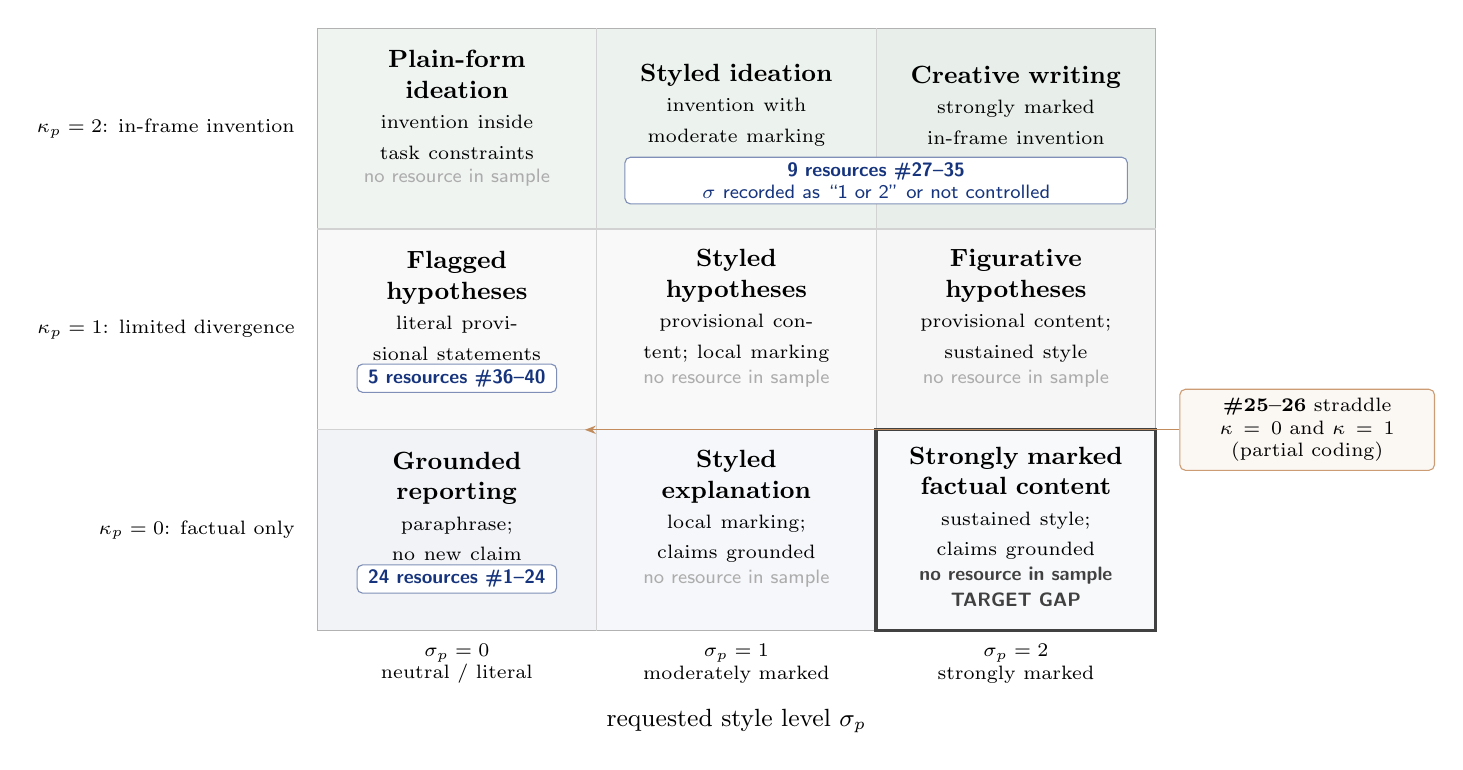
\begin{tikzpicture}[x=1cm,y=1cm,font=\small]
  \def\cw{3.55}
  \def\rh{2.55}
  \fill[clrB!6] (0,0) rectangle (\cw,\rh);
  \fill[clrB!4] (\cw,0) rectangle (2*\cw,\rh);
  \fill[clrB!3] (2*\cw,0) rectangle (3*\cw,\rh);
  \fill[gray!5] (0,\rh) rectangle (\cw,2*\rh);
  \fill[gray!5] (\cw,\rh) rectangle (2*\cw,2*\rh);
  \fill[gray!7] (2*\cw,\rh) rectangle (3*\cw,2*\rh);
  \fill[clrLD!7] (0,2*\rh) rectangle (\cw,3*\rh);
  \fill[clrLD!8] (\cw,2*\rh) rectangle (2*\cw,3*\rh);
  \fill[clrLD!10] (2*\cw,2*\rh) rectangle (3*\cw,3*\rh);
  \draw[gray!60] (0,0) rectangle (3*\cw,3*\rh);
  \draw[gray!35] (\cw,0)--(\cw,3*\rh);
  \draw[gray!35] (2*\cw,0)--(2*\cw,3*\rh);
  \draw[gray!35] (0,\rh)--(3*\cw,\rh);
  \draw[gray!35] (0,2*\rh)--(3*\cw,2*\rh);
  \draw[very thick,clrG] (2*\cw,0) rectangle (3*\cw,\rh);
  \tikzset{
    cell/.style={align=center,text width=3.15cm},
    full/.style={rectangle,rounded corners=2pt,draw=clrB!55,fill=white,
      font=\scriptsize\sffamily\bfseries,text=clrB,inner xsep=4pt,inner ysep=2pt},
    empty/.style={font=\scriptsize\sffamily,text=gray!65}}
  \node[cell] at (0.5*\cw,0.5*\rh+0.30)
    {\textbf{Grounded reporting}\\{\scriptsize paraphrase; no new claim}};
  \node[full] at (0.5*\cw,0.5*\rh-0.62) {24 resources \textbf{\#1--24}};
  \node[cell] at (1.5*\cw,0.5*\rh+0.30)
    {\textbf{Styled\\explanation}\\{\scriptsize local marking; claims grounded}};
  \node[empty] at (1.5*\cw,0.5*\rh-0.62) {no resource in sample};
  \node[cell] at (2.5*\cw,0.5*\rh+0.34)
    {\textbf{Strongly marked\\factual content}\\{\scriptsize sustained style; claims grounded}};
  \node[empty,text=clrG,font=\scriptsize\sffamily\bfseries] at (2.5*\cw,0.5*\rh-0.58)
    {no resource in sample};
  \node[font=\scriptsize\sffamily\bfseries,text=clrG] at (2.5*\cw,0.5*\rh-0.88) {TARGET GAP};
  \node[cell] at (0.5*\cw,1.5*\rh+0.30)
    {\textbf{Flagged\\hypotheses}\\{\scriptsize literal provisional statements}};
  \node[full] at (0.5*\cw,1.5*\rh-0.62) {5 resources \textbf{\#36--40}};
  \node[cell] at (1.5*\cw,1.5*\rh+0.30)
    {\textbf{Styled\\hypotheses}\\{\scriptsize provisional content; local marking}};
  \node[empty] at (1.5*\cw,1.5*\rh-0.62) {no resource in sample};
  \node[cell] at (2.5*\cw,1.5*\rh+0.30)
    {\textbf{Figurative hypotheses}\\{\scriptsize provisional content; sustained style}};
  \node[empty] at (2.5*\cw,1.5*\rh-0.62) {no resource in sample};
  \node[cell] at (0.5*\cw,2.5*\rh+0.30)
    {\textbf{Plain-form ideation}\\{\scriptsize invention inside task constraints}};
  \node[empty] at (0.5*\cw,2.5*\rh-0.62) {no resource in sample};
  \node[cell] at (1.5*\cw,2.5*\rh+0.30)
    {\textbf{Styled ideation}\\{\scriptsize invention with moderate marking}};
  \node[cell] at (2.5*\cw,2.5*\rh+0.30)
    {\textbf{Creative writing}\\{\scriptsize strongly marked in-frame invention}};
  \node[full,text width=6.1cm,align=center] at (2*\cw,2.5*\rh-0.66)
    {9 resources \textbf{\#27--35}\\
     \mdseries$\sigma$ recorded as ``1 or 2'' or not controlled};
  \node[draw=clrO!60,fill=clrO!5,rounded corners=2pt,font=\scriptsize,
        text width=3.0cm,align=center,anchor=west] (part) at (3*\cw+0.3,\rh)
    {\textbf{\#25--26} straddle\\$\kappa=0$ and $\kappa=1$\\(partial coding)};
  \draw[clrO!70,-{Stealth[length=4pt,width=3pt]}]
    (part.west) -- (\cw-0.15,\rh);
  \node[font=\scriptsize,align=center] at (0.5*\cw,-0.42){$\sigma_p=0$\\neutral / literal};
  \node[font=\scriptsize,align=center] at (1.5*\cw,-0.42){$\sigma_p=1$\\moderately marked};
  \node[font=\scriptsize,align=center] at (2.5*\cw,-0.42){$\sigma_p=2$\\strongly marked};
  \node[font=\small] at (1.5*\cw,-1.15){requested style level $\sigma_p$};
  \node[font=\scriptsize,anchor=east] at (-0.16,0.5*\rh){$\kappa_p=0$: factual only};
  \node[font=\scriptsize,anchor=east] at (-0.16,1.5*\rh){$\kappa_p=1$: limited divergence};
  \node[font=\scriptsize,anchor=east] at (-0.16,2.5*\rh){$\kappa_p=2$: in-frame invention};
\end{tikzpicture}}
\caption{\textbf{Task-design space, with the forty mapped resources placed in it.}
The grid crosses the three permission levels $\kappa_p\in\{0,1,2\}$ with the three requested style levels $\sigma_p\in\{0,1,2\}$.
Cell names are illustrative task profiles; the badges report where the resources of Appendix~\ref{app:mapping} fall under our coding, indexed by the numbering used there.
Nine resources (\#27--35) appear as one badge spanning two cells because their protocols do not separate $\sigma=1$ from $\sigma=2$, and two adjacent resources (\#25--26) receive partial codes spanning two permission levels.
The counts are occupancy in a purposive sample, not prevalence in the field, and cell shading encodes no quantity.
The outlined $\sigma_p=2,\ \kappa_p=0$ cell is the diagnostic gap: strongly marked language under a factual-only contract is the combination in which a style-sensitive verifier would misfire, and no sampled resource tests it.}
\label{fig:profiles}
\end{figure*}

\section{Worked Cases}\label{sec:cases}

The following cases illustrate how one or more contract components affect the analysis.
They are conceptual demonstrations rather than measurements: each states what a labeling rule should return, and none reports what any system did return.
Each case names the resource type in which its contrast arises, with numbers referring to the index of Appendix~\ref{app:mapping}.
Cases A--D instantiate contrasts that occur in resource types present in the sample, so a reader can locate the setting even though the strings are ours.
Case E has no such setting, for a reason Figure~\ref{fig:profiles} makes visible: it lives in the $\sigma=2,\ \kappa=0$ cell, which no sampled resource occupies.
Where the sample is empty, a constructed example is the only kind available.

\paragraph{Case A: changing the reference evidence}
In XSum, an extrinsic but factual summary statement may be absent from the source document while being correct against external evidence \citep{maynez_faithfulness_2020}.
\emph{Fixed:} the response span, the recovered claim, and an empty permission scope.
\emph{Changed:} $O$ is either the source document or an external evidence set.
\emph{Outcome:} the claim receives \Hall\ when the source does not support it and \SUP\ when the external evidence entails it.
\emph{Lesson:} the evidence source must be explicit.

\paragraph{Case B: changing the discourse frame}
\emph{Setting:} the contrast between a factual-QA resource such as PopQA or TriviaQA (\#3, \#5), coded $\kappa=0$, and a story-generation resource such as LitBench or Short Story (\#28, \#29), coded $\kappa=2$.
The two families are evaluated by different protocols, and no sampled resource evaluates one wording under both.
\emph{Fixed:} the constructed surface string in Figure~\ref{fig:flip}.
\emph{Changed:} the prompt changes both the discourse frame and the permission scope.
\emph{Outcome:} the historical prompt yields a real-world claim labeled \Hall, whereas the fiction prompt yields an in-frame claim labeled \LD.
\emph{Lesson:} identical wording need not express an identical contextualized claim.

\paragraph{Case C: changing the epistemic presentation}
\emph{Setting:} grounded question answering over product documentation, the task type DelucionQA evaluates (\#15), where the provided manual routinely leaves a question undetermined.
That resource scores support against the manual and does not separately score how an undetermined answer is presented, which is the field our $\mu$ column records as ``not scored''.
Suppose the available evidence cannot determine whether a tool supports several input formats.
\emph{Fixed:} the core proposition that the tool supports several formats and the evidence-unknown state.
\emph{Changed:} the required epistemic presentation and the asserted status.
\emph{Outcome:} a categorical assertion receives \Hall, whereas ``the tool may support several formats, but this requires version-specific verification'' can receive \LD\ under a hypothesis-generation contract.
\emph{Lesson:} presentation requirements determine whether permitted uncertainty is communicated correctly.

\paragraph{Case D: testing a scope boundary}
\emph{Setting:} creative-writing evaluation of the kind LitBench, WritingBench, and Art-or-Artifice conduct (\#28, \#30, \#31), all coded $\kappa=2$ with an implicit story frame and $\mu$ not separated.
The scope boundary we probe is precisely the one those protocols leave implicit; we use an invented person because attributing fabricated conduct to a real individual is not something a published example should do.
\emph{Fixed:} a prompt that permits invention inside a declared fictional frame.
\emph{Changed:} the target of the claim moves from a fictional entity to a real named person presented as real history.
\emph{Outcome:} the second claim falls outside $\Gamma_p$ and receives \Hall.
\emph{Lesson:} in-frame invention does not license every real-world assertion.

\paragraph{Case E: changing claim type under requested style level}
\emph{Setting:} none available.
This case requires a resource that requests $\sigma=2$ while holding the contract to $\kappa=0$, and Figure~\ref{fig:profiles} shows that cell empty.
Creative resources that reach $\sigma=2$ (\#27--35) all sit at $\kappa=2$, and every resource coded $\kappa=0$ (\#1--24) assumes neutral wording.
The case is therefore constructed, and the absence of an alternative is the gap this paper argues should be filled.
\emph{Fixed:} the scientific evidence, the empty permission scope, and the recovered canonical claims of Table~\ref{tab:contracts}.
\emph{Changed:} a neutral realization is replaced by a strongly marked one.
\emph{Outcome:} the claims remain \SUP, while the mixed span additionally receives $z=1$ and \SV.
\emph{Lesson:} a literal pseudo-claim extracted from the figurative wording is a claim-recovery error, not a factual defect in the matched claim.

Together, Cases A--E isolate the role of reference evidence, discourse frame, epistemic presentation, permission scope, and style-conditioned claim recovery.

\section{Research Agenda}\label{sec:agenda}

The framework motivates seven connected priorities that form a validation sequence: annotation, benchmark construction, pipeline diagnosis, aggregation, mitigation, generalization, and extension to agentic settings.

\textbf{1. Contract annotation, inference, and reliability.}
Benchmarks should annotate the reference evidence $O_p$, the three-level requested style level $\sigma_p$, the observed style level $\widehat\sigma$, permission level $\kappa_p$, scope, and epistemic presentation separately.
A public codebook should define contextualized claims, claim-preserving style variation, and evidence states.
Reliability should be reported for each layer, and annotator disagreement should be preserved when prompts are ambiguous.
Contract inference must also resolve conflicts among user prompts, system instructions, domain rules, and safety policies.
Multi-turn studies should track when a clarification, correction, or role instruction changes $\TC(p)$ instead of treating the first prompt as a fixed contract for the whole dialogue.

Annotating four contract fields, an observed style level, and a claim-level label costs more than annotating a binary factuality judgment.
We take the objection seriously: a scheme too expensive to apply would not be applied.
Two properties of the contract limit what the added annotation actually costs.
The contract is a property of the task rather than of the response, so $O_p$, $\sigma_p$, $\Gamma_p$, and $\mu_p$ are annotated once per prompt and amortized over every response and every model evaluated on it, while only the claim-level label scales with the number of responses.
Most existing resources are also single-valued on three of the four fields, as our mapping shows: a benchmark coded $\kappa=0$ throughout needs one declaration at the resource level, not one annotation per item.
The remaining cost, claim-level adjudication, is one the field already pays, since decompose-then-verify pipelines require it whether or not a contract is recorded \citep{min_factscore_2023,metropolitansky_claimify_2025}.
The diagnostic benchmark of priority~2 is the genuinely expensive object, because its fields must vary by design.
We accept that cost, and note that it falls on one instrument rather than on every evaluation that uses the framework.

\textbf{2. Factorial benchmark design.}
A diagnostic benchmark should cross $\kappa_p\in\{0,1,2\}$ with $\sigma_p\in\{0,1,2\}$ while holding canonical claims as stable as possible.
Expert-adjudicated triplets should express the same claim in neutral, moderately marked, and strongly marked forms.
Within each cell, targeted contrasts should vary $\Gamma_p$ and $\mu_p$ to distinguish permission breadth from permission scope and required presentation.
Evaluation should report span type, observed-style accuracy, \SV\ placement, claim-set equivalence, evidence state, and claim-level label.
A successful evaluator need not produce identical raw extractions across styles; it should recover equivalent canonical claims and stable labels after matching.
The mapping in Appendix~\ref{app:mapping} provides possible comparators, not a validated benchmark.

\textbf{3. Style-robust claim recovery and verification.}
Claim extractors and verifiers should be stress-tested on metaphor, analogy, irony, narrative voice, hypotheses, and declared fiction.
Experiments should separate span-type errors, claim-recovery errors, evidence errors, and contract-label errors so that a final \Hall\ label can be traced to the stage that produced it.
Comparisons across extraction, natural-language-inference, retrieval, and LLM-judge pipelines should report both accuracy and calibration under each $\sigma_p$ level.
The central test is whether matched canonical claims keep stable evidence states and labels when only their permitted surface realization changes.

\textbf{4. Response-level aggregation.}
A complete response $y$ requires a response-level assessment $R(y\mid p)$ built from its claim-level labels and other task outcomes.
Research should compare transparent aggregation rules, including the proportion of \Hall\ claims, a worst-case rule, severity-weighted scoring, and task-utility-aware scoring.
Each aggregate should be reported together with the underlying claim-label distribution, claim coverage, style compliance, and sensitivity to the chosen rule.
Different contracts may justify different aggregations; for example, one severe unsupported medical claim and one harmless fictional detail should not be treated as interchangeable events.
We leave the design and validation of an optimal contract-aware $R$ open rather than building it into the claim-level definition.

\textbf{5. Mitigation that preserves licensed divergence and factual style.}
Retrieval, verification, abstention, and constrained decoding should be assessed on three outcomes: reducing \Hall\ under grounded contracts, preserving useful \LD\ under permissive contracts, and preserving supported content at $\sigma_p=1$ or $2$.
Usefulness should remain a separate score with its own uncertainty \citep{acar_creativity_2019,marco_reader_2025}.
Results should expose trade-offs among these outcomes, for example through per-contract scores or Pareto comparisons, rather than through one aggregate hallucination rate.
This would test whether a mitigation method makes a model more reliable without making it uniformly literal, overly cautious, or less useful in creative tasks.

\textbf{6. Generalization across domains, languages, and interactions.}
The three-level $\sigma_p$ and $\kappa_p$ scales should be tested in high-stakes factual domains, educational explanation, journalism, scientific communication, brainstorming, and fiction.
Multilingual work should examine whether style markers, hedges, and genre conventions lead to comparable annotations across languages and cultures.
Interactive studies should also measure whether users understand the model's epistemic presentation and whether contract-aware outputs improve trust calibration and task utility.

\textbf{7. Contracts in agentic and tool-using settings.}
The framework as stated is single-turn and prompt-anchored, and the assumptions that make it tractable there break first when a model plans, calls tools, and delegates.
The most consequential is that $O_p$ is fixed at the outset.
An agent constitutes its own reference evidence through retrieval and tool calls during the trajectory, so a claim is judged against evidence that did not exist when the task was issued, and an evaluation must record when $O_p$ was fixed as well as what it contained.
Contracts also multiply and can conflict, because a task decomposes into subtasks: a planning step may legitimately operate at $\kappa=2$ while the step that reports results to the user must operate at $\kappa=0$, so a divergence that is licensed where it is produced becomes a violation where it is surfaced.
Finally, $\mu_p$ acquires non-epistemic consequences, since what one component reports as established rather than conjectured determines what a downstream component does; a presentation failure then propagates into action, not only into a reader's belief.
Existing tool-use benchmarks evaluate task success and do not separate these fields \citep{zhuang_toolqa_2023}, which makes contract inference across a trajectory an open problem rather than an application of the single-turn case.


\section{Discussion}\label{sec:discussion}

\subsection{Evaluation implications}

No single rate should conflate factual support, contractual permission, stylistic marking, severity, and usefulness.
At claim level, each recovered claim receives \SUP, \Hall, or \LD; at span level, \SV\ records an orthogonal stylistic contribution; and at response level, $R(y\mid p)$ applies a stated aggregation rule.
A response may still be too conservative for a creative task even when it contains no \Hall.
Likewise, a response may remain supported but reduce a requested $\sigma_p=2$ style to neutral prose.
These are output-level task-compliance failures, not new claim labels.
Conversely, satisfying $\sigma_p=2$ does not excuse a fabricated claim under a factual-only contract.
Reporting claim-level labels, their aggregation rule, and style compliance separately makes ``creative and factual when required'' an evaluable target.

The framework also separates the claim label from severity.
A false drug dose and a wrong trivia date can both receive \Hall, but their costs differ.
Severity should weight the penalty after the contractual claim label rather than determine whether a violation occurred.

\paragraph{Avoiding indiscriminate suppression}
Formal work suggests that some errors remain possible for sufficiently general models operating with incomplete evidence \citep{kalai_calibrated_2024,xu_hallucination_2024,banerjee_llms_2024}, although this does not imply a constant deployment error rate \citep{suzuki_negligible_2025}.
The operational consequence is narrower: suppressing every departure from observed evidence would also suppress hypotheses and in-frame invention.
Evaluation should instead distinguish reductions in unlicensed departures (\Hall), preservation of licensed ones (\LD), and retention of supported content at the requested style level \citep{banerjee_does_2025,sun_hallucinating_2024,he_shakespearean_2025}.

\subsection{Scope and validation priorities}

This position paper presents an operational starting point and makes its validation path explicit.
First, contract specification necessarily includes normative choices about the relevant evidence, permission boundary, and authority of user, system, safety, legal, and domain instructions.
Making these choices explicit is a feature of the framework; future multi-turn work can extend the prompt-centered formulation to contracts that change during dialogue.

Second, the three-level $\sigma_p$ and $\kappa_p$ scales are working operational scales intended to support testable comparisons.
Human annotation studies can refine their thresholds while $\Gamma_p$ and $\mu_p$ preserve task-specific distinctions that a single ordinal level cannot express.
Metaphor, irony, hypothesis, and fiction provide demanding but informative tests for claim extraction, \LD\ annotation, and style robustness.
The claim-level rule is therefore specified now, while alternative response-level aggregation rules $R(y\mid p)$ remain open for direct empirical comparison.

Third, the purposive, author-coded mapping establishes a concrete coverage pattern in the selected resources.
A larger systematic review, independent recoding, and a public codebook would strengthen estimates of how often each truth-contract profile occurs in the broader literature.
These boundaries define the next validation steps, and they leave the paper's central distinction fully testable: evidential support, content permission, and requested style.


\section{Conclusion}\label{sec:conclusion}

In this position paper, we argued that hallucination should be evaluated relative to a task's truth contract rather than treated as a context-free property of a sentence.
Concretely, hallucination is a claim-level label relative to a task's reference evidence, requested style, permission scope, and required epistemic presentation.
The truth contract $\TC(p)=(O_p,\sigma_p,\Gamma_p,\mu_p)$ makes these variables explicit without changing what is true.
An evidence-unknown claim receives \LD\ only when its content, scope, and presentation are permitted; otherwise it receives \Hall.
Usefulness, severity, style compliance, and response-level aggregation remain separate assessments.

In our purposive sample of forty evaluation resources, these variables are rarely represented together, and the worked cases illustrate their distinct roles.
The main validation priorities are reliable contract annotation, style-robust claim matching, transparent aggregation, and mitigation that reduces \Hall\ while preserving \LD\ and factually grounded style.

\appendix

\appendixsection{Additional Diagnostics and Response-Level Aggregation}%
\makeatletter\def\@currentlabel{A}\makeatother\label{app:diagnostics}

Section~\ref{sec:framework} defines the truth contract, span types, and claim-label rule.
This appendix records the additional diagnostics needed for an empirical implementation.

\paragraph{Style-stability test}
Consider three expert-adjudicated realizations $s_0,s_1,s_2$ produced under task contexts that differ only in requested style, with $\sigma_{p_0}=0$, $\sigma_{p_1}=1$, and $\sigma_{p_2}=2$.
After neutral normalization and one-to-one adjudicated matching, let $\mathcal C^*(s_i,p_i)$ denote each set of canonical claims.
Equality below means that the matched sets contain the same factual commitments, not that their surface strings are identical.
For claim-preserving variants with fixed $O_p$, $\Gamma_p$, and $\mu_p$, the desired stability condition is
\[
\mathcal C^*(s_0,p_0)=\mathcal C^*(s_1,p_1)=\mathcal C^*(s_2,p_2),
\qquad
V(c_j^*\mid p_0)=V(c_j^*\mid p_1)=V(c_j^*\mid p_2)
\]
for every matched canonical claim $c_j^*$.
Observed style levels and \SV\ flags may legitimately differ.

\begin{itemize}
  \item \emph{Span-type error}: incorrect assignment of other, SV-only, claim-only, or mixed.
  \item \emph{Claim-recovery error}: a canonical claim is dropped, added spuriously, or changed during neutral paraphrase.
  \item \emph{Claim-label instability}: claim-matched variants receive different labels when $O_p$, $\Gamma_p$, and $\mu_p$ are fixed.
  \item \emph{Aggregation sensitivity}: the response-level ranking changes when the evaluator changes the rule used to combine claim labels.
\end{itemize}

The first three diagnostics require a benchmark distribution and expert-adjudicated claim matches before they can be estimated as error rates.
Claim-label instability is an error only when $O_p$, $\Gamma_p$, and $\mu_p$ all remain fixed.
When a permission field changes, the same evidence-unknown claim may intentionally change from \Hall\ to \LD; this is contract dependence, not relative truth.

For a complete response $y$, an evaluation should publish the claim-label distribution, observed style compliance, and any severity or usefulness weights before reporting $R(y\mid p)$.
Comparisons should report sensitivity to plausible aggregation rules rather than present one rule as uniquely determined.

The running example makes the stakes of that sensitivity concrete.
Figure~\ref{fig:prompt-to-claim} yields one \SUP, one \SUP\ with an \SV\ flag, one \LD, and one \Hall.
Under a worst-case rule the response is a failure, since it contains an unlicensed claim.
Under a proportional rule three of its four claims are contract-conforming, and the response reads as largely acceptable with one identified defect.
Under a severity-weighted rule the verdict depends on how a fabricated attribution to a named individual is weighted against three conforming claims.
We do not adjudicate between these rules.
We note only that the claim-level labels are the same in all three cases, that the reported number is not, and that an evaluation reporting only the number leaves its reader unable to reconstruct which of the three questions was answered.

\appendixsection{Resource Mapping}%
\makeatletter\def\@currentlabel{B}\makeatother\label{app:mapping}
\renewcommand*{\theHtable}{B.\arabic{table}}

Tables~\ref{tab:full-mapping-factual-a}--\ref{tab:full-mapping-creative} list the forty resources used in the purposive mapping.
Each row shows the six recorded fields: reference evidence $O$, requested style $\sigma$, permission level $\kappa$, permission scope $\Gamma$, presentation requirement $\mu$, and whether the resource tests stylistic marking as a factuality-measurement error (ME).
The $\sigma$ column uses the paper's three levels; ``not controlled'' means that style is neither fixed nor scored as a distinct variable.
The $\kappa$ column uses $0$ for factual only, $1$ for limited divergence, and $2$ for in-frame invention.
``Implicit'' means that a value is inferred from task design, ``partial'' means that only part of a component is represented, and ``not separated'' or ``not scored'' means that the protocol does not evaluate the field independently.
Thus, an implicit $\kappa=2$ code does not mean that a benchmark explicitly annotates its permission fields; it means that invention is needed or accepted by the task although its permission boundary is not independently evaluated.
The task profiles are coarse author annotations inferred from the original protocols, not labels reported by those resources.
They require a public codebook and independent recoding before release as a validated dataset.

\begin{table*}[t]
\centering
\footnotesize
\setlength{\tabcolsep}{5pt}
\renewcommand{\arraystretch}{1.08}
\caption{\textbf{Factuality and faithfulness resources in the purposive mapping (part I).}
The table shows the five structural dimensions recorded in the mapping: $O$, $\sigma$, $\kappa$, $\Gamma$, and $\mu$.
The recurring author-coded profile is fixed evidence, implicit $\sigma=0$, inferred $\kappa=0$, no applicable permission scope, and no separate scoring of $\mu$.}
\label{tab:full-mapping-factual-a}
\begin{tabularx}{0.99\linewidth}{@{}P{0.22\textwidth}P{0.28\textwidth}P{0.18\textwidth}Y@{}}
\toprule
\textbf{Resource} & \textbf{Task and $O$} & \textbf{$\sigma$ / $\kappa$} & \textbf{$\Gamma$ / $\mu$}\\
\midrule
\multicolumn{4}{l}{\textbf{Strict factuality and faithfulness}}\\
1.~FEVER \citep{thorne_fever_2018} & Fact checking\newline $O$: Wikipedia evidence & $\sigma$: implicit 0\newline $\kappa$: implicit 0 & $\Gamma$: n/a\newline $\mu$: not scored\\
2.~TruthfulQA \citep{lin_truthfulqa_2022} & Factual QA\newline $O$: external factual reference & $\sigma$: implicit 0\newline $\kappa$: implicit 0 & $\Gamma$: n/a\newline $\mu$: not scored\\
3.~PopQA \citep{mallen_when_2023} & Long-tail QA\newline $O$: Wikidata & $\sigma$: implicit 0\newline $\kappa$: implicit 0 & $\Gamma$: n/a\newline $\mu$: not scored\\
4.~SimpleQA \citep{wei_measuring_2024} & Factual QA\newline $O$: external factual reference & $\sigma$: implicit 0\newline $\kappa$: implicit 0 & $\Gamma$: n/a\newline $\mu$: not scored\\
5.~TriviaQA \citep{joshi_triviaqa_2017} & Reading QA\newline $O$: evidence documents & $\sigma$: implicit 0\newline $\kappa$: implicit 0 & $\Gamma$: n/a\newline $\mu$: not scored\\
6.~DefAn \citep{rahman_defan_2024} & Factual QA\newline $O$: external factual reference & $\sigma$: implicit 0\newline $\kappa$: implicit 0 & $\Gamma$: n/a\newline $\mu$: not scored\\
7.~HaluEval \citep{li_halueval_2023} & QA and summarization\newline $O$: world/reference context & $\sigma$: implicit 0\newline $\kappa$: implicit 0 & $\Gamma$: n/a\newline $\mu$: not scored\\
8.~FactBench \citep{bayat_factbench_2024} & Factual QA\newline $O$: retrieved evidence & $\sigma$: implicit 0\newline $\kappa$: implicit 0 & $\Gamma$: n/a\newline $\mu$: not scored\\
9.~HalluLens \citep{bang_hallulens_2025} & Factual QA\newline $O$: task-specific evidence & $\sigma$: implicit 0\newline $\kappa$: implicit 0 & $\Gamma$: n/a\newline $\mu$: not scored\\
10.~FRANK \citep{pagnoni_understanding_2021} & Summarization\newline $O$: source documents & $\sigma$: implicit 0\newline $\kappa$: implicit 0 & $\Gamma$: n/a\newline $\mu$: not scored\\
11.~QAGS \citep{wang_asking_2020} & Summarization\newline $O$: source documents & $\sigma$: implicit 0\newline $\kappa$: implicit 0 & $\Gamma$: n/a\newline $\mu$: not scored\\
12.~SummEval \citep{fabbri_summeval_2021} & Summarization\newline $O$: source documents & $\sigma$: implicit 0\newline $\kappa$: implicit 0 & $\Gamma$: n/a\newline $\mu$: not scored\\
13.~XSum \citep{narayan_xsum_2018} & Summarization\newline $O$: BBC source & $\sigma$: implicit 0\newline $\kappa$: implicit 0 & $\Gamma$: n/a\newline $\mu$: not scored\\
\bottomrule
\end{tabularx}
\end{table*}

\clearpage
\begin{table*}[t]
\centering
\footnotesize
\setlength{\tabcolsep}{5pt}
\renewcommand{\arraystretch}{1.08}
\caption{\textbf{Factuality, faithfulness, and adjacent resources in the purposive mapping (part II).}
The coding follows Table~\ref{tab:full-mapping-factual-a} and shows the same five structural dimensions.
For adjacent resources, ``partial'' indicates that a protocol captures some task constraints without independently representing both permission fields.}
\label{tab:full-mapping-factual-b}
\begin{tabularx}{0.99\linewidth}{@{}P{0.22\textwidth}P{0.28\textwidth}P{0.18\textwidth}Y@{}}
\toprule
\textbf{Resource} & \textbf{Task and $O$} & \textbf{$\sigma$ / $\kappa$} & \textbf{$\Gamma$ / $\mu$}\\
\midrule
\multicolumn{4}{l}{\textbf{Strict factuality and faithfulness (continued)}}\\
14.~CNN/DailyMail \citep{hermann_teaching_2015} & Summarization\newline $O$: news source & $\sigma$: implicit 0\newline $\kappa$: implicit 0 & $\Gamma$: n/a\newline $\mu$: not scored\\
15.~DelucionQA \citep{sadat_delucionqa_2023} & Domain QA\newline $O$: manuals & $\sigma$: implicit 0\newline $\kappa$: implicit 0 & $\Gamma$: n/a\newline $\mu$: not scored\\
16.~HalluQA \citep{cheng_evaluating_2023} & Long-form QA\newline $O$: external factual reference & $\sigma$: implicit 0\newline $\kappa$: implicit 0 & $\Gamma$: n/a\newline $\mu$: not scored\\
17.~BIG-Bench \citep{srivastava_beyond_2023} & Multi-task reasoning\newline $O$: task gold & $\sigma$: implicit 0\newline $\kappa$: implicit 0 & $\Gamma$: n/a\newline $\mu$: not scored\\
18.~BIG-Bench Hard \citep{suzgun_challenging_2023} & Reasoning\newline $O$: task gold & $\sigma$: implicit 0\newline $\kappa$: implicit 0 & $\Gamma$: n/a\newline $\mu$: not scored\\
19.~CR-LLM \citep{li_cr-llm_2024} & Concept reasoning\newline $O$: gold concepts/context & $\sigma$: implicit 0\newline $\kappa$: implicit 0 & $\Gamma$: n/a\newline $\mu$: not scored\\
20.~HotpotQA \citep{yang_hotpotqa_2018} & Multi-hop QA\newline $O$: Wikipedia & $\sigma$: implicit 0\newline $\kappa$: implicit 0 & $\Gamma$: n/a\newline $\mu$: not scored\\
21.~HypoTermQA \citep{uluoglakci_hypotermqa_2024} & Hypothetical QA\newline $O$: task/world reference & $\sigma$: implicit 0\newline $\kappa$: implicit 0 & $\Gamma$: n/a\newline $\mu$: not scored\\
22.~HalluRAG \citep{ridder_hallurag_2025} & RAG QA\newline $O$: retrieved Wikipedia & $\sigma$: implicit 0\newline $\kappa$: implicit 0 & $\Gamma$: n/a\newline $\mu$: not scored\\
23.~ToolQA \citep{zhuang_toolqa_2023} & Tool-use QA\newline $O$: tools and APIs & $\sigma$: implicit 0\newline $\kappa$: implicit 0 & $\Gamma$: n/a\newline $\mu$: not scored\\
24.~RealTime QA \citep{kasai_realtime_2024} & Real-time QA\newline $O$: current evidence & $\sigma$: implicit 0\newline $\kappa$: implicit 0 & $\Gamma$: n/a\newline $\mu$: not scored\\
\midrule
\multicolumn{4}{l}{\textbf{Closest intent and hallucination taxonomies}}\\
25.~FaithQA \citep{hao_faithqa_2025} & Intent verification\newline $O$: query constraints & $\sigma$: 0 dominant; not controlled\newline $\kappa$: partial, 0 or 1 & $\Gamma$: partial (query constraints)\newline $\mu$: not separated\\
26.~HIC-Bench \citep{yang_hicbench_2025} & Hallucination typing\newline $O$: task-dependent & $\sigma$: 0 dominant; not controlled\newline $\kappa$: partial, 0 to 2 & $\Gamma$: partial (task types)\newline $\mu$: not separated\\
\bottomrule
\end{tabularx}
\end{table*}

\clearpage
\begin{table*}[t]
\centering
\footnotesize
\setlength{\tabcolsep}{5pt}
\renewcommand{\arraystretch}{1.08}
\caption{\textbf{Creativity and constrained problem-solving resources in the purposive mapping.}
Creative-writing resources tend toward $\sigma=1$ or $2$ with task-implied $\kappa=2$, whereas divergent-thinking tasks often leave style uncontrolled.
Constrained problem-solving resources mostly use neutral form and partial $\kappa=1$ constraints.
Scope is coded only when a task frame or constraint set supplies it; no sampled protocol separately scores $\mu$ in our coding.}
\label{tab:full-mapping-creative}
\begin{tabularx}{0.99\linewidth}{@{}P{0.22\textwidth}P{0.28\textwidth}P{0.18\textwidth}Y@{}}
\toprule
\textbf{Resource} & \textbf{Task and $O$} & \textbf{$\sigma$ / $\kappa$} & \textbf{$\Gamma$ / $\mu$}\\
\midrule
\multicolumn{4}{l}{\textbf{Creative generation and divergent thinking}}\\
27.~CreativityPrism \citep{hou_creativityprism_2025} & Multi-task creativity\newline $O$: task-specific rubrics & $\sigma$: mixed; not isolated\newline $\kappa$: implicit 2 & $\Gamma$: implicit task frame\newline $\mu$: not separated\\
28.~LitBench \citep{fein_litbench_2025} & Story evaluation\newline $O$: human preferences & $\sigma$: implicit 1 or 2\newline $\kappa$: implicit 2 & $\Gamma$: implicit story frame\newline $\mu$: not separated\\
29.~Short Story \citep{ismayilzada_evaluating_2025} & Story generation\newline $O$: semantic/human criteria & $\sigma$: implicit 1 or 2\newline $\kappa$: implicit 2 & $\Gamma$: implicit story frame\newline $\mu$: not separated\\
30.~WritingBench \citep{wu_writingbench_2025} & Creative writing\newline $O$: rubric/human criteria & $\sigma$: scored 1 or 2\newline $\kappa$: implicit 2 & $\Gamma$: implicit task frame\newline $\mu$: not separated\\
31.~Art-or-Artifice / TTCW \citep{chakrabarty_art_2024} & Creative writing\newline $O$: expert rubric & $\sigma$: implicit 1 or 2\newline $\kappa$: implicit 2 & $\Gamma$: implicit story frame\newline $\mu$: not separated\\
32.~Automated DT scoring \citep{organisciak_beyond_2023} & Divergent thinking\newline $O$: automated rubric & $\sigma$: not controlled\newline $\kappa$: implicit 2 & $\Gamma$: implicit task frame\newline $\mu$: not separated\\
33.~Verbal Creativity \citep{dinu_testing_2025} & Divergent thinking\newline $O$: TTCT & $\sigma$: not controlled\newline $\kappa$: implicit 2 & $\Gamma$: implicit task frame\newline $\mu$: not separated\\
34.~Automated Creativity \citep{li_automated_2025} & Creative writing\newline $O$: reference texts & $\sigma$: implicit 1 or 2\newline $\kappa$: implicit 2 & $\Gamma$: implicit task frame\newline $\mu$: not separated\\
35.~Hallucinating Narratives \citep{sun_hallucinating_2024} & Controlled story/reasoning\newline $O$: mixed evidence/rubric & $\sigma$: implicit 1 or 2\newline $\kappa$: partial 2 & $\Gamma$: partial (mixed frame)\newline $\mu$: not separated\\
\midrule
\multicolumn{4}{l}{\textbf{Constrained creative problem solving}}\\
36.~MacGyver \citep{tian_macgyver_2025} & Problem solving\newline $O$: human feasibility & $\sigma$: implicit 0\newline $\kappa$: partial 1 & $\Gamma$: partial (feasibility)\newline $\mu$: not separated\\
37.~EscapeBench \citep{qian_escapebench_2025} & Agent puzzles\newline $O$: environment state & $\sigma$: implicit 0\newline $\kappa$: partial 1 & $\Gamma$: partial (correctness)\newline $\mu$: not separated\\
38.~CreativEval \citep{delorenzo_creativeval_2024} & Code generation\newline $O$: specification/tests & $\sigma$: implicit 0\newline $\kappa$: partial 1 & $\Gamma$: partial (specification)\newline $\mu$: not separated\\
39.~NeoCoder \citep{lu_benchmarking_2025} & Code generation\newline $O$: unit tests & $\sigma$: implicit 0\newline $\kappa$: partial 1 & $\Gamma$: partial (tests)\newline $\mu$: not separated\\
40.~Math Creativity \citep{ye_assessing_2024} & Math problem solving\newline $O$: human soundness & $\sigma$: implicit 0\newline $\kappa$: partial 1 & $\Gamma$: partial (soundness)\newline $\mu$: not separated\\
\bottomrule
\end{tabularx}
\end{table*}

\clearpage
\bibliography{references}

\end{document}

